% Options for packages loaded elsewhere
\PassOptionsToPackage{unicode}{hyperref}
\PassOptionsToPackage{hyphens}{url}
%
\documentclass[
]{book}
\usepackage{lmodern}
\usepackage{amssymb,amsmath}
\usepackage{ifxetex,ifluatex}
\ifnum 0\ifxetex 1\fi\ifluatex 1\fi=0 % if pdftex
  \usepackage[T1]{fontenc}
  \usepackage[utf8]{inputenc}
  \usepackage{textcomp} % provide euro and other symbols
\else % if luatex or xetex
  \usepackage{unicode-math}
  \defaultfontfeatures{Scale=MatchLowercase}
  \defaultfontfeatures[\rmfamily]{Ligatures=TeX,Scale=1}
\fi
% Use upquote if available, for straight quotes in verbatim environments
\IfFileExists{upquote.sty}{\usepackage{upquote}}{}
\IfFileExists{microtype.sty}{% use microtype if available
  \usepackage[]{microtype}
  \UseMicrotypeSet[protrusion]{basicmath} % disable protrusion for tt fonts
}{}
\makeatletter
\@ifundefined{KOMAClassName}{% if non-KOMA class
  \IfFileExists{parskip.sty}{%
    \usepackage{parskip}
  }{% else
    \setlength{\parindent}{0pt}
    \setlength{\parskip}{6pt plus 2pt minus 1pt}}
}{% if KOMA class
  \KOMAoptions{parskip=half}}
\makeatother
\usepackage{xcolor}
\IfFileExists{xurl.sty}{\usepackage{xurl}}{} % add URL line breaks if available
\IfFileExists{bookmark.sty}{\usepackage{bookmark}}{\usepackage{hyperref}}
\hypersetup{
  pdftitle={Life Contingencies: The Mathematics, Statistics, and Economics of Life Insurance},
  pdfauthor={An open text authored by the Actuarial Community},
  hidelinks,
  pdfcreator={LaTeX via pandoc}}
\urlstyle{same} % disable monospaced font for URLs
\usepackage{color}
\usepackage{fancyvrb}
\newcommand{\VerbBar}{|}
\newcommand{\VERB}{\Verb[commandchars=\\\{\}]}
\DefineVerbatimEnvironment{Highlighting}{Verbatim}{commandchars=\\\{\}}
% Add ',fontsize=\small' for more characters per line
\usepackage{framed}
\definecolor{shadecolor}{RGB}{248,248,248}
\newenvironment{Shaded}{\begin{snugshade}}{\end{snugshade}}
\newcommand{\AlertTok}[1]{\textcolor[rgb]{0.94,0.16,0.16}{#1}}
\newcommand{\AnnotationTok}[1]{\textcolor[rgb]{0.56,0.35,0.01}{\textbf{\textit{#1}}}}
\newcommand{\AttributeTok}[1]{\textcolor[rgb]{0.77,0.63,0.00}{#1}}
\newcommand{\BaseNTok}[1]{\textcolor[rgb]{0.00,0.00,0.81}{#1}}
\newcommand{\BuiltInTok}[1]{#1}
\newcommand{\CharTok}[1]{\textcolor[rgb]{0.31,0.60,0.02}{#1}}
\newcommand{\CommentTok}[1]{\textcolor[rgb]{0.56,0.35,0.01}{\textit{#1}}}
\newcommand{\CommentVarTok}[1]{\textcolor[rgb]{0.56,0.35,0.01}{\textbf{\textit{#1}}}}
\newcommand{\ConstantTok}[1]{\textcolor[rgb]{0.00,0.00,0.00}{#1}}
\newcommand{\ControlFlowTok}[1]{\textcolor[rgb]{0.13,0.29,0.53}{\textbf{#1}}}
\newcommand{\DataTypeTok}[1]{\textcolor[rgb]{0.13,0.29,0.53}{#1}}
\newcommand{\DecValTok}[1]{\textcolor[rgb]{0.00,0.00,0.81}{#1}}
\newcommand{\DocumentationTok}[1]{\textcolor[rgb]{0.56,0.35,0.01}{\textbf{\textit{#1}}}}
\newcommand{\ErrorTok}[1]{\textcolor[rgb]{0.64,0.00,0.00}{\textbf{#1}}}
\newcommand{\ExtensionTok}[1]{#1}
\newcommand{\FloatTok}[1]{\textcolor[rgb]{0.00,0.00,0.81}{#1}}
\newcommand{\FunctionTok}[1]{\textcolor[rgb]{0.00,0.00,0.00}{#1}}
\newcommand{\ImportTok}[1]{#1}
\newcommand{\InformationTok}[1]{\textcolor[rgb]{0.56,0.35,0.01}{\textbf{\textit{#1}}}}
\newcommand{\KeywordTok}[1]{\textcolor[rgb]{0.13,0.29,0.53}{\textbf{#1}}}
\newcommand{\NormalTok}[1]{#1}
\newcommand{\OperatorTok}[1]{\textcolor[rgb]{0.81,0.36,0.00}{\textbf{#1}}}
\newcommand{\OtherTok}[1]{\textcolor[rgb]{0.56,0.35,0.01}{#1}}
\newcommand{\PreprocessorTok}[1]{\textcolor[rgb]{0.56,0.35,0.01}{\textit{#1}}}
\newcommand{\RegionMarkerTok}[1]{#1}
\newcommand{\SpecialCharTok}[1]{\textcolor[rgb]{0.00,0.00,0.00}{#1}}
\newcommand{\SpecialStringTok}[1]{\textcolor[rgb]{0.31,0.60,0.02}{#1}}
\newcommand{\StringTok}[1]{\textcolor[rgb]{0.31,0.60,0.02}{#1}}
\newcommand{\VariableTok}[1]{\textcolor[rgb]{0.00,0.00,0.00}{#1}}
\newcommand{\VerbatimStringTok}[1]{\textcolor[rgb]{0.31,0.60,0.02}{#1}}
\newcommand{\WarningTok}[1]{\textcolor[rgb]{0.56,0.35,0.01}{\textbf{\textit{#1}}}}
\usepackage{longtable,booktabs}
% Correct order of tables after \paragraph or \subparagraph
\usepackage{etoolbox}
\makeatletter
\patchcmd\longtable{\par}{\if@noskipsec\mbox{}\fi\par}{}{}
\makeatother
% Allow footnotes in longtable head/foot
\IfFileExists{footnotehyper.sty}{\usepackage{footnotehyper}}{\usepackage{footnote}}
\makesavenoteenv{longtable}
\usepackage{graphicx,grffile}
\makeatletter
\def\maxwidth{\ifdim\Gin@nat@width>\linewidth\linewidth\else\Gin@nat@width\fi}
\def\maxheight{\ifdim\Gin@nat@height>\textheight\textheight\else\Gin@nat@height\fi}
\makeatother
% Scale images if necessary, so that they will not overflow the page
% margins by default, and it is still possible to overwrite the defaults
% using explicit options in \includegraphics[width, height, ...]{}
\setkeys{Gin}{width=\maxwidth,height=\maxheight,keepaspectratio}
% Set default figure placement to htbp
\makeatletter
\def\fps@figure{htbp}
\makeatother
\setlength{\emergencystretch}{3em} % prevent overfull lines
\providecommand{\tightlist}{%
  \setlength{\itemsep}{0pt}\setlength{\parskip}{0pt}}
\setcounter{secnumdepth}{5}
\usepackage{booktabs}
\usepackage{pdfpages}
\setcounter{secnumdepth}{2}
\let\oldmaketitle\maketitle
\AtBeginDocument{\let\maketitle\relax}
\usepackage{booktabs}
\usepackage{longtable}
\usepackage{array}
\usepackage{multirow}
\usepackage{wrapfig}
\usepackage{float}
\usepackage{colortbl}
\usepackage{pdflscape}
\usepackage{tabu}
\usepackage{threeparttable}
\usepackage{threeparttablex}
\usepackage[normalem]{ulem}
\usepackage{makecell}
\usepackage{xcolor}
\usepackage[]{natbib}
\bibliographystyle{econPeriod}

\title{Life Contingencies: The Mathematics, Statistics, and Economics of Life Insurance}
\author{An open text authored by the Actuarial Community}
\date{}

\begin{document}
\maketitle

\thispagestyle{empty}
%\begin{center}
%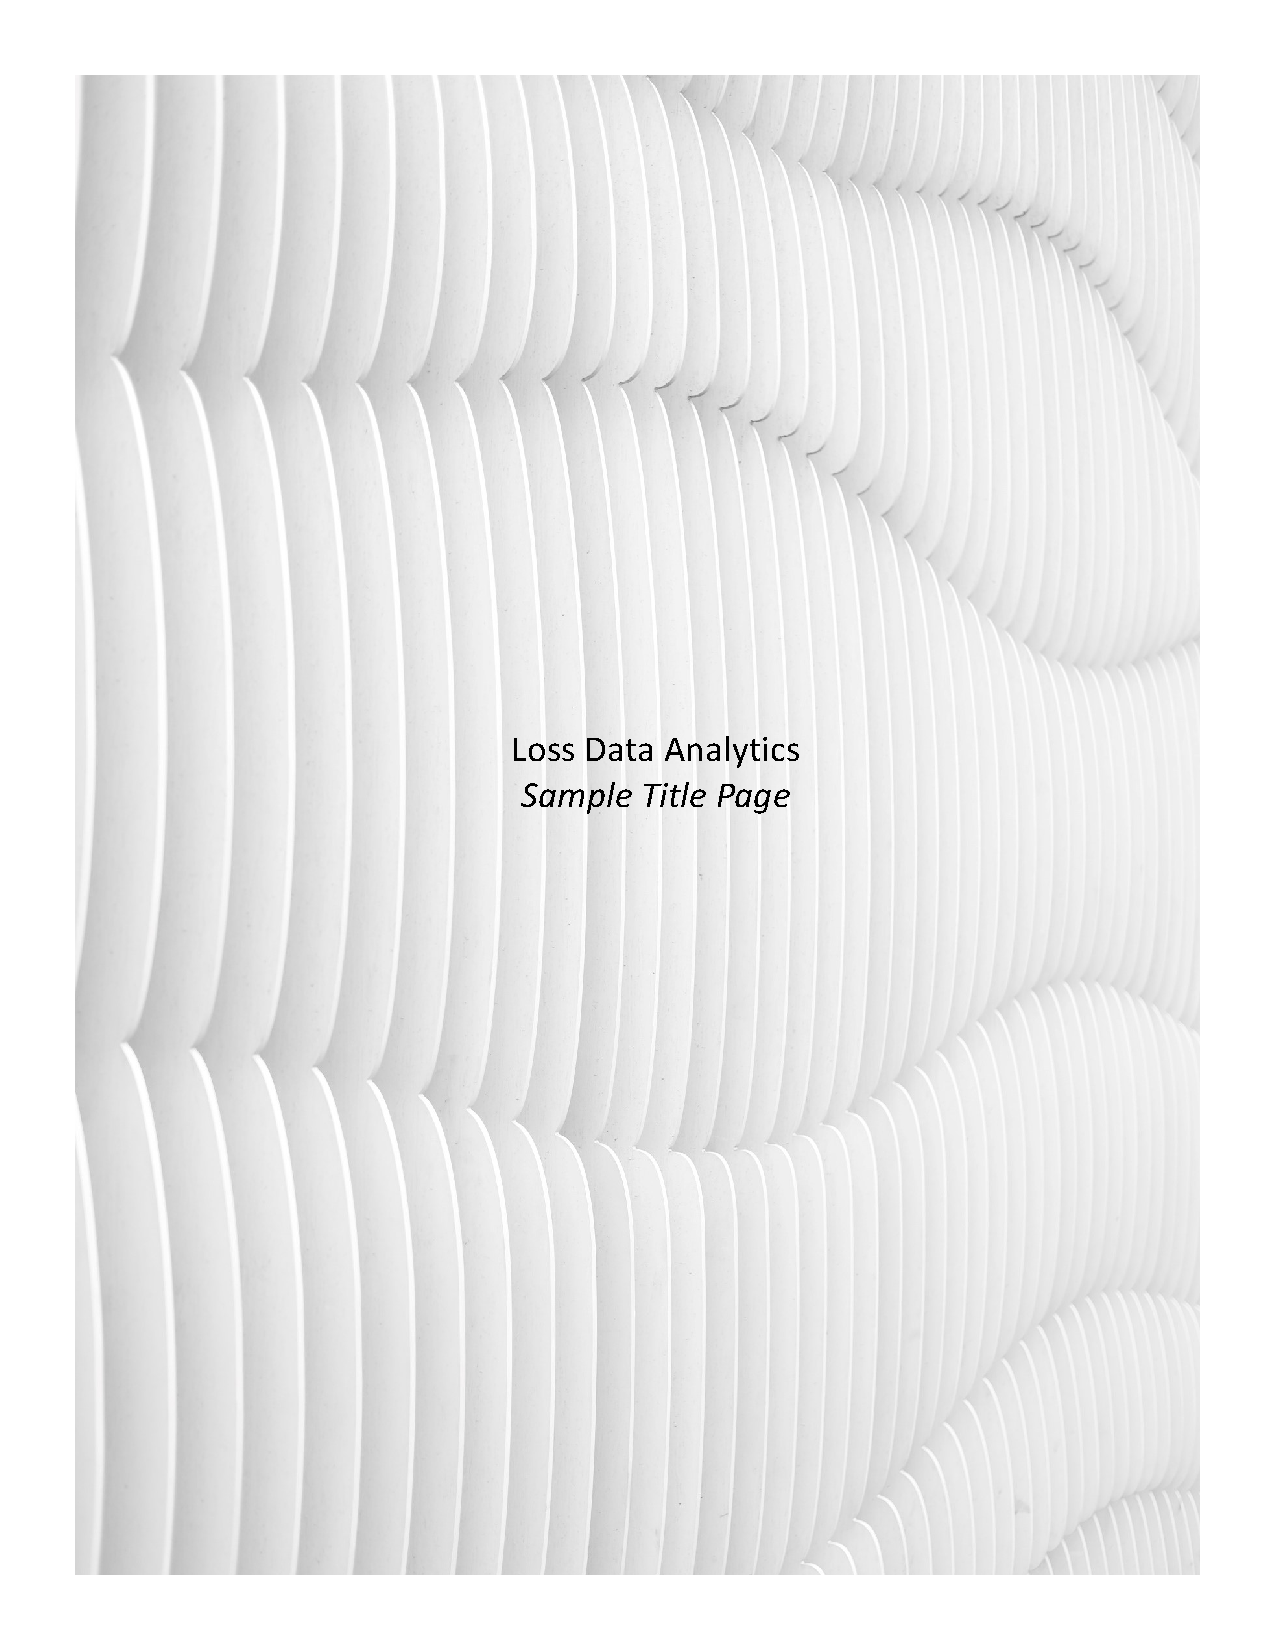
\includepdf{title.pdf}
%\end{center}

\let\maketitle\oldmaketitle
\maketitle

{
\setcounter{tocdepth}{2}
\tableofcontents
}
\hypertarget{preface}{%
\chapter*{Preface}\label{preface}}
\addcontentsline{toc}{chapter}{Preface}

\emph{Date: 25 April 2022}

\hypertarget{book-description}{%
\subsubsection*{Book Description}\label{book-description}}
\addcontentsline{toc}{subsubsection}{Book Description}

Like the companion book \href{https://openacttexts.github.io/Loss-Data-Analytics/index.html}{Loss Data Analytics}, this book on life contingencies will be an interactive, online, freely available text.

\begin{itemize}
\tightlist
\item
  The online version will contain many interactive objects (quizzes, computer demonstrations, interactive graphs, video, and the like) to promote \emph{deeper learning}. A subset of the book will be available for \emph{offline} reading in pdf and EPUB formats.
\item
  Will focus on data and statistical aspects of life contingent events.
\item
  Will emphasize cash flow fundamentals, an approach that allows users to easily adapt approaches to handle complex products.
\item
  This modular approach emphasizing data and cash flow fundamentals has additional advantages:

  \begin{itemize}
  \tightlist
  \item
    computational aspects become practically relevant through spreadsheet (e.g., \texttt{Microsoft\ Excel}) and numerical (\texttt{R}) examples, and
  \item
    an emphasis on the foundations provides an easy entry point for learners who wish an introduction to the field.
  \end{itemize}
\end{itemize}

\hypertarget{how-will-the-text-be-used}{%
\subsubsection*{How will the text be used?}\label{how-will-the-text-be-used}}
\addcontentsline{toc}{subsubsection}{How will the text be used?}

This book will be useful in actuarial curricula worldwide. Our primary \textbf{target audience} is second or third year undergraduates with little to no experience in insurance. Learners may be international; although the book will be in English, we do not expect knowledge of native idiosyncrasies that might be used in the classroom. It will cover the learning objectives of the major actuarial organizations. Thus, it will be suitable for classroom use at universities as well as for use by independent learners seeking to pass professional actuarial examinations.

A secondary audience is the actuarial practitioner (perhaps international) who wishes to retool and learn about modern approaches in the risk management of life contingent events. Thus, the text will also be useful for the continuing professional development of actuaries and other professionals in insurance and related financial risk management industries.

\hypertarget{why-is-this-good-for-the-profession}{%
\subsubsection*{Why is this good for the profession?}\label{why-is-this-good-for-the-profession}}
\addcontentsline{toc}{subsubsection}{Why is this good for the profession?}

An online text is a type of open educational resource (OER). One important benefit of an OER is that it equalizes access to knowledge, thus permitting a broader community to learn about the actuarial profession. Moreover, it has the capacity to engage viewers through active learning that deepens the learning process, producing analysts more capable of solid actuarial work.

Why is this good for students and teachers and others involved in the learning process? Cost is often cited as an important factor for students and teachers in textbook selection (see a recent post on the \href{https://www.aei.org/publication/the-new-era-of-the-400-college-textbook-which-is-part-of-the-unsustainable-higher-education-bubble/}{\$400 textbook}). Students will also appreciate the ability to ``carry the book around'' on their mobile devices.

\hypertarget{life-contingent-calculations}{%
\subsubsection*{Life Contingent Calculations}\label{life-contingent-calculations}}
\addcontentsline{toc}{subsubsection}{Life Contingent Calculations}

Life contingences is a quantitative discipline, enjoying the rigor and discipline of mathematics. Like any mathematical discipline, one traditionally learns about it through the development of formulaic expressions, that is, their proofs, special cases, analysis of special features, and so on. Users of this text find that we do not shy away from presenting summaries of main conclusions using formulaic expressions. Nonetheless, rather than developing insights from mathematical proofs of the primary findings, we demonstrate their impact through short illustrative examples and links to practical applications.

As with other sources that introduce life contingencies, we utilize spreadsheets extensively. In our teaching, we find that spreadsheets are useful for communication and dynamically visualizing results as they evolve over time. However, unlike other sources, we supplement this with approaches that emphasize programming; in this text, we use \texttt{R}. Programming methods such as through \texttt{R} (and Python, another good candidate) easily accommodate more complex situations that require more computing and, moreover, are built to graphically portray results in an attractive fashion. Analytics, the process of using data to make decisions, is enjoying tremendous attention from many industries; this is certainly true of in data-driven fields that use life contingent methods. By working with data and using programming methods such as \texttt{R} in the study of life contingences, users see the connections within many fields that support the actuarial science discpline. Instruction may emphasize any one of the three approaches, traditional mathematical development, spreadsheets, or a computing approach. However, this text contains all three as we believe that future generations of actuaries need to be familiar with all of these different ways to analyze, and communicate, problems that can be solved using life contingent methods.

\hypertarget{project-goal}{%
\subsubsection*{Project Goal}\label{project-goal}}
\addcontentsline{toc}{subsubsection}{Project Goal}

The project goal is to have the actuarial community author our textbooks in a collaborative fashion. To get involved, please visit our
\href{https://sites.google.com/a/wisc.edu/loss-data-analytics/}{Open Actuarial Textbooks Project Site}.

\hypertarget{acknowledgements}{%
\section*{Acknowledgements}\label{acknowledgements}}
\addcontentsline{toc}{section}{Acknowledgements}

We acknowledge the Society of Actuaries for permission to use problems from their examinations.

We thank Rob Hyndman, Monash University, for allowing us to use his excellent style files to produce the online version of the book.

We thank Yihui Xie and his colleagues at \href{https://www.rstudio.com/}{Rstudio} for the \href{https://bookdown.org/yihui/bookdown/}{R bookdown} package that allows us to produce this book.

We also wish to acknowledge the support and sponsorship of the \href{http://www.blackactuaries.org/}{International Association of Black Actuaries} in our joint efforts to provide actuarial educational content to all.


\includegraphics[width=0.25\textwidth,height=\textheight]{Figures/IABA.png}

\hypertarget{contributors}{%
\section*{Contributors}\label{contributors}}
\addcontentsline{toc}{section}{Contributors}

The project goal is to have the actuarial community author our textbooks in a collaborative fashion. The following contributors have taken a leadership role in developing \emph{Life Contingencies}.

\begin{itemize}
\tightlist
\item
  \textbf{Vali Asimit}
\item
  \textbf{Dani Bauer}
\item
  \textbf{Adam Butt}
\item
  \textbf{Edward (Jed) Frees}
\item
  \textbf{Emiliano Valdez}
\end{itemize}

\hypertarget{for-our-readers}{%
\section*{For our Readers}\label{for-our-readers}}
\addcontentsline{toc}{section}{For our Readers}

Like any book, we have a set of notations and conventions. It will probably save you time if you regularly visit our Appendix Chapter \ref{C:NotationConventionLC} to get used to ours.

Freely available, interactive textbooks represent a new venture in actuarial education and we need your input. Although a lot of effort has gone into the development, we expect hiccoughs. Please let your instructor know about opportunities for improvement, write us through our project site, or contact chapter contributors directly with suggested improvements.

\hypertarget{exercises}{%
\chapter{Exercises}\label{exercises}}

\hypertarget{chapter-4-exercises}{%
\section{Chapter 4 Exercises}\label{chapter-4-exercises}}

\hypertarget{section-4.3-exercises}{%
\subsubsection*{Section 4.3 Exercises}\label{section-4.3-exercises}}
\addcontentsline{toc}{subsubsection}{Section 4.3 Exercises}

\textbf{Exercise 4.3.1. Actuarial Present Values for Select and Ultimate Tables}. The select and ultimate tables introduced in Section \ref{Sec:SelectionAdverse} are complicated -- is such complexity is warranted in practice? To get insights into this question, in this exercise you will compare actuarial present values derived from select and ultimate mortality to those from only ultimate mortality. To be specific, we focus consider whole life insurance for using the female Canadian experience introduced in Section \ref{Sec:SelectionAdverse}; the data are available in Appendix Section \ref{Sec:CanadianSelect}.

For these data,

\begin{enumerate}
\def\labelenumi{\alph{enumi}.}
\tightlist
\item
  produce \(A_x\) for \(x=50, \ldots, 65\) using an interest rate of \(i=0.04\) based on

  \begin{enumerate}
  \def\labelenumii{\roman{enumii}.}
  \tightlist
  \item
    select and ultimate mortality
  \item
    ultimate mortality
  \end{enumerate}
\item
  compare these two sequences of actuarial present values by calculating their ratio.
\item
  repeat parts (a) and (b) using an interest rate \(i=0.02\).
\end{enumerate}

To give you a feel for the results, Figure \ref{fig:SelUlt1} summarizes the results.



\begin{figure}

{\centering 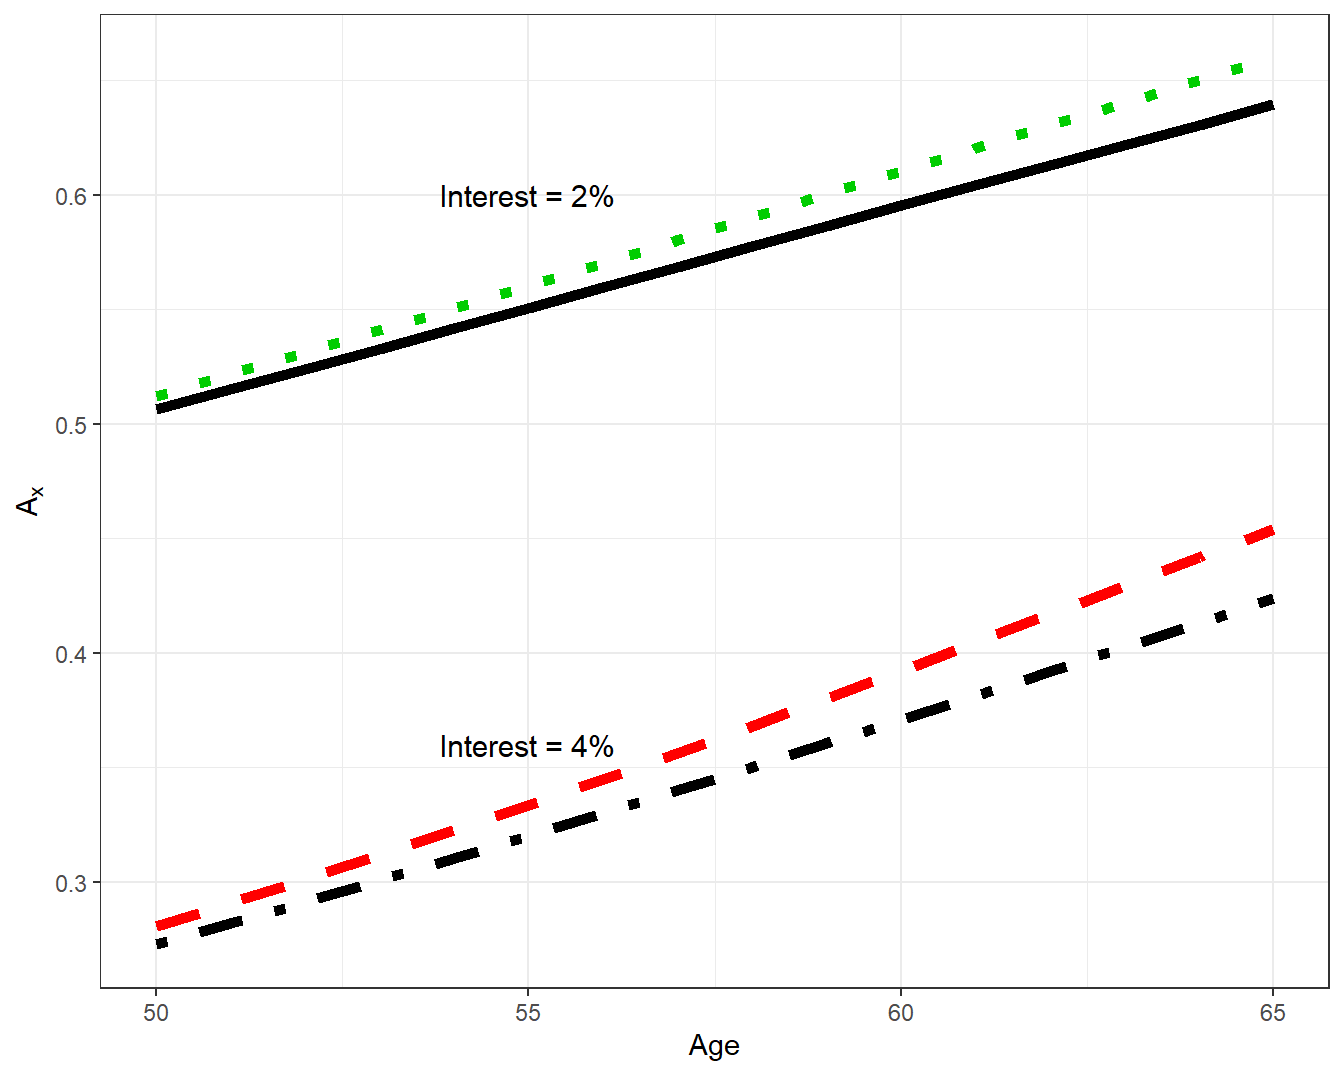
\includegraphics[width=0.6\linewidth]{LifeCon_files/figure-latex/SelUlt1-1} 

}

\caption{\textbf{Life Insurance APV by Age, Interest, and Mortality Type}. A plot of life insurance actuarial present value \(A_x\) by age \(x\). The top two lines are based on \(i=0.02\), the bottom two based on \(i=0.04\). For each pair, the top line uses ultimate mortality, the bottom line is based on select and ultimate mortality}\label{fig:SelUlt1}
\end{figure}

Exercise 4.3.1 Answer

\leavevmode\hypertarget{toggleTheory.Exer4.3.1}{}%
\textbackslash begin\{table\}

\textbackslash caption\{\label{tab:unnamed-chunk-5}Comparison of Life Insurance APVs, Interest is 4\%\}
\centering

\begin{tabular}[t]{l|r|r|r|r|r|r|r|r}
\hline
Age & 50 & 51 & 52 & 53 & 54 & 55 & 56 & 57\\
\hline
Select2 and Ultimate, i=4\% & 0.2729 & 0.282 & 0.2913 & 0.3007 & 0.3104 & 0.3201 & 0.33 & 0.3401\\
\hline
Ultimate, i=4\% & 0.2808 & 0.2908 & 0.3011 & 0.3117 & 0.3225 & 0.3336 & 0.3449 & 0.3564\\
\hline
Ratio & 0.9716 & 0.9695 & 0.9673 & 0.9649 & 0.9624 & 0.9598 & 0.957 & 0.9542\\
\hline
Age & 58 & 59 & 60 & 61 & 62 & 63 & 64 & 65\\
\hline
Select and Ultimate, i=4\% & 0.3502 & 0.3605 & 0.3709 & 0.3814 & 0.3919 & 0.4025 & 0.4132 & 0.424\\
\hline
Ultimate, i=4\% & 0.3682 & 0.3801 & 0.3923 & 0.4046 & 0.417 & 0.4294 & 0.4417 & 0.454\\
\hline
Ratio & 0.9513 & 0.9484 & 0.9455 & 0.9425 & 0.9398 & 0.9375 & 0.9355 & 0.934\\
\hline
\end{tabular}

\textbackslash end\{table\}

\textbackslash begin\{table\}

\textbackslash caption\{\label{tab:unnamed-chunk-6}Comparison of Life Insurance APVs, Interest is 2\%\}
\centering

\begin{tabular}[t]{l|r|r|r|r|r|r|r|r}
\hline
Age & 50 & 51 & 52 & 53 & 54 & 55 & 56 & 57\\
\hline
Select and Ultimate, i=2\% & 0.5063 & 0.5151 & 0.524 & 0.5329 & 0.5418 & 0.5507 & 0.5596 & 0.5686\\
\hline
Ultimate, i=2\% & 0.5122 & 0.5217 & 0.5312 & 0.5408 & 0.5506 & 0.5604 & 0.5702 & 0.5802\\
\hline
Ratio & 0.9885 & 0.9875 & 0.9864 & 0.9853 & 0.9841 & 0.9828 & 0.9814 & 0.98\\
\hline
Age & 58 & 59 & 60 & 61 & 62 & 63 & 64 & 65\\
\hline
Select and Ultimate, i=2\% & 0.5775 & 0.5864 & 0.5953 & 0.6042 & 0.6131 & 0.6219 & 0.6307 & 0.6394\\
\hline
Ultimate, i=2\% & 0.5901 & 0.6002 & 0.6102 & 0.6203 & 0.6303 & 0.6402 & 0.6499 & 0.6595\\
\hline
Ratio & 0.9786 & 0.9771 & 0.9756 & 0.9741 & 0.9727 & 0.9715 & 0.9704 & 0.9695\\
\hline
\end{tabular}

\textbackslash end\{table\}

Exercise 4.3.1 Solution using R Code

\hypertarget{toggleCode.Exer4.3.1A}{}
\begin{Shaded}
\begin{Highlighting}[]
\NormalTok{CanadianSelUlt <-}\StringTok{ }\KeywordTok{read.csv}\NormalTok{(}\StringTok{"Data/CanadianFemaleSelectRead.csv"}\NormalTok{, }\DataTypeTok{stringsAsFactors =} \OtherTok{FALSE}\NormalTok{)}

\NormalTok{temp <-}\StringTok{ }\NormalTok{CanadianSelUlt[}\DecValTok{131}\OperatorTok{:}\DecValTok{201}\NormalTok{,}\DecValTok{1}\OperatorTok{:}\DecValTok{2}\NormalTok{]}
\NormalTok{temp1 <-}\StringTok{ }\KeywordTok{as.matrix}\NormalTok{(temp)}
\NormalTok{CanadianUlt50 <-}\StringTok{ }\KeywordTok{matrix}\NormalTok{(}\KeywordTok{as.numeric}\NormalTok{(temp1), }\DataTypeTok{ncol=}\DecValTok{2}\NormalTok{)}
\KeywordTok{colnames}\NormalTok{(CanadianUlt50) <-}\StringTok{ }\KeywordTok{c}\NormalTok{(}\StringTok{"Age"}\NormalTok{, }\StringTok{"qx_Ult"}\NormalTok{)}
\KeywordTok{rownames}\NormalTok{(CanadianUlt50) <-}\StringTok{ }\OtherTok{NULL}

\NormalTok{tempSel <-}\StringTok{ }\NormalTok{CanadianSelUlt[}\DecValTok{51}\OperatorTok{:}\DecValTok{81}\NormalTok{,]}
\NormalTok{tempSel1 <-}\StringTok{ }\KeywordTok{as.matrix}\NormalTok{(tempSel)}

\NormalTok{CanadianSel50 <-}\StringTok{ }\KeywordTok{matrix}\NormalTok{(}\KeywordTok{as.numeric}\NormalTok{(tempSel1), }\DataTypeTok{ncol=}\KeywordTok{ncol}\NormalTok{(tempSel))}
\KeywordTok{rownames}\NormalTok{(CanadianSel50) <-}\StringTok{ }\OtherTok{NULL}

\NormalTok{CanadianSel50.toUlt <-}\StringTok{ }\KeywordTok{matrix}\NormalTok{(}\DecValTok{1}\NormalTok{, }\DataTypeTok{nrow =} \KeywordTok{nrow}\NormalTok{(CanadianSel50), }\DataTypeTok{ncol =} \DecValTok{120-50}\OperatorTok{+}\DecValTok{1}\NormalTok{)}
\NormalTok{CanadianSel50.toUlt[}\DecValTok{1}\OperatorTok{:}\KeywordTok{nrow}\NormalTok{(CanadianSel50),}\DecValTok{1}\OperatorTok{:}\KeywordTok{ncol}\NormalTok{(CanadianSel50)] <-}\StringTok{ }\NormalTok{CanadianSel50}

\ControlFlowTok{for}\NormalTok{ (irow }\ControlFlowTok{in}\NormalTok{ (}\DecValTok{1}\OperatorTok{:}\KeywordTok{nrow}\NormalTok{(CanadianSel50)) )\{}
\ControlFlowTok{for}\NormalTok{ (icol }\ControlFlowTok{in}\NormalTok{ (}\DecValTok{1}\OperatorTok{:}\StringTok{ }\NormalTok{(}\DecValTok{120-50-15}\OperatorTok{-}\NormalTok{irow)) )\{}
\NormalTok{  CanadianSel50.toUlt[irow,}\DecValTok{1}\OperatorTok{+}\DecValTok{15}\OperatorTok{+}\NormalTok{icol ] <-}\StringTok{ }\NormalTok{CanadianUlt50[irow}\OperatorTok{+}\DecValTok{14}\OperatorTok{+}\NormalTok{icol,}\DecValTok{2}\NormalTok{]}
\NormalTok{   \}}
\NormalTok{\}}

\CommentTok{#  Actuarial Present Value Calculations}
\NormalTok{APV.Ult <-}\StringTok{ }\ControlFlowTok{function}\NormalTok{(xage, q.x, }\DataTypeTok{int=}\FloatTok{0.00}\NormalTok{)\{}
\NormalTok{  v =}\StringTok{ }\DecValTok{1}\OperatorTok{/}\NormalTok{(}\DecValTok{1}\OperatorTok{+}\NormalTok{int)}
\NormalTok{  num =}\StringTok{ }\KeywordTok{length}\NormalTok{(xage)}
\NormalTok{  A.x <-}\StringTok{ }\DecValTok{0}\OperatorTok{*}\NormalTok{xage ->}\StringTok{ }\NormalTok{add.x ->}\StringTok{ }\NormalTok{e.x}
\NormalTok{  A.x[num] =}\StringTok{ }\NormalTok{v}\OperatorTok{*}\NormalTok{q.x[num]}
\NormalTok{  add.x[num] =}\StringTok{ }\DecValTok{1} \OperatorTok{+}\StringTok{ }\NormalTok{(}\DecValTok{1}\OperatorTok{-}\NormalTok{q.x[num])}\OperatorTok{/}\NormalTok{(int }\OperatorTok{+}\StringTok{ }\FloatTok{1e-12}\NormalTok{)}
\NormalTok{  e.x[num] =}\StringTok{ }\DecValTok{1}\OperatorTok{-}\NormalTok{q.x[num]}
  \ControlFlowTok{for}\NormalTok{ (i }\ControlFlowTok{in} \DecValTok{1}\OperatorTok{:}\NormalTok{(num}\DecValTok{-1}\NormalTok{))\{}
\NormalTok{    A.x[num}\OperatorTok{-}\NormalTok{i] =}\StringTok{ }\NormalTok{v}\OperatorTok{*}\NormalTok{q.x[num}\OperatorTok{-}\NormalTok{i] }\OperatorTok{+}\StringTok{ }\NormalTok{v}\OperatorTok{*}\NormalTok{(}\DecValTok{1}\OperatorTok{-}\NormalTok{q.x[num}\OperatorTok{-}\NormalTok{i])}\OperatorTok{*}\NormalTok{A.x[num}\OperatorTok{-}\NormalTok{i}\OperatorTok{+}\DecValTok{1}\NormalTok{]}
\NormalTok{    add.x[num}\OperatorTok{-}\NormalTok{i] =}\StringTok{ }\DecValTok{1} \OperatorTok{+}\StringTok{ }\NormalTok{v}\OperatorTok{*}\NormalTok{(}\DecValTok{1}\OperatorTok{-}\NormalTok{q.x[num}\OperatorTok{-}\NormalTok{i])}\OperatorTok{*}\NormalTok{add.x[num}\OperatorTok{-}\NormalTok{i}\OperatorTok{+}\DecValTok{1}\NormalTok{] }
\NormalTok{    e.x[num}\OperatorTok{-}\NormalTok{i] =}\StringTok{  }\NormalTok{(}\DecValTok{1}\OperatorTok{-}\NormalTok{q.x[num}\OperatorTok{-}\NormalTok{i])}\OperatorTok{*}\NormalTok{(}\DecValTok{1}\OperatorTok{+}\NormalTok{e.x[num}\OperatorTok{-}\NormalTok{i}\OperatorTok{+}\DecValTok{1}\NormalTok{])}
\NormalTok{    \}}
\NormalTok{  tablelife <-}\StringTok{ }\KeywordTok{cbind}\NormalTok{(xage,q.x,A.x,add.x,e.x)}
  \KeywordTok{return}\NormalTok{(tablelife)}
\NormalTok{\}}
\NormalTok{AxUlt04 <-}\StringTok{ }\KeywordTok{APV.Ult}\NormalTok{(}\DataTypeTok{xage=}\NormalTok{ CanadianUlt50[,}\DecValTok{1}\NormalTok{], }\DataTypeTok{q.x=}\NormalTok{CanadianUlt50[,}\DecValTok{2}\NormalTok{], }\DataTypeTok{int=}\FloatTok{0.04}\NormalTok{)[,}\DecValTok{3}\NormalTok{]}
\NormalTok{AxUlt04}\FloatTok{.5065}\NormalTok{ <-}\StringTok{ }\NormalTok{AxUlt04[}\DecValTok{1}\OperatorTok{:}\DecValTok{16}\NormalTok{]}
\NormalTok{AxUlt02 <-}\StringTok{ }\KeywordTok{APV.Ult}\NormalTok{(}\DataTypeTok{xage=}\NormalTok{ CanadianUlt50[,}\DecValTok{1}\NormalTok{], }\DataTypeTok{q.x=}\NormalTok{CanadianUlt50[,}\DecValTok{2}\NormalTok{], }\DataTypeTok{int=}\FloatTok{0.02}\NormalTok{)[,}\DecValTok{3}\NormalTok{]}
\NormalTok{AxUlt02}\FloatTok{.5065}\NormalTok{ <-}\StringTok{ }\NormalTok{AxUlt02[}\DecValTok{1}\OperatorTok{:}\DecValTok{16}\NormalTok{]}

\CommentTok{#  Actuarial Present Value Calculations}

\NormalTok{APV.Sel <-}\StringTok{ }\ControlFlowTok{function}\NormalTok{(}\DataTypeTok{int=}\FloatTok{0.00}\NormalTok{)\{}
\NormalTok{AxSel04 <-}\StringTok{ }\KeywordTok{rep}\NormalTok{(}\DecValTok{0}\NormalTok{, }\DecValTok{16}\NormalTok{)}
\NormalTok{  v =}\StringTok{ }\DecValTok{1}\OperatorTok{/}\NormalTok{(}\DecValTok{1}\OperatorTok{+}\NormalTok{int)}
\ControlFlowTok{for}\NormalTok{ (iage }\ControlFlowTok{in} \DecValTok{1}\OperatorTok{:}\DecValTok{16}\NormalTok{)\{}
\CommentTok{#iage =2}
\NormalTok{  AxSel04[iage] =}\StringTok{  }\NormalTok{v}\OperatorTok{*}\NormalTok{CanadianSel50.toUlt[iage, }\DecValTok{2}\NormalTok{]}
\NormalTok{kpx =}\StringTok{ }\DecValTok{1}
  \ControlFlowTok{for}\NormalTok{ (k }\ControlFlowTok{in} \DecValTok{1}\OperatorTok{:}\NormalTok{(}\KeywordTok{ncol}\NormalTok{(CanadianSel50.toUlt)}\OperatorTok{-}\DecValTok{2}\NormalTok{)) \{}
\NormalTok{    kpx =}\StringTok{ }\NormalTok{kpx}\OperatorTok{*}\NormalTok{(}\DecValTok{1}\OperatorTok{-}\NormalTok{CanadianSel50.toUlt[iage, k}\OperatorTok{+}\DecValTok{1}\NormalTok{])}
\NormalTok{   AxSel04[iage] =}\StringTok{  }\NormalTok{AxSel04[iage] }\OperatorTok{+}\StringTok{ }\NormalTok{v}\OperatorTok{**}\NormalTok{(k}\OperatorTok{+}\DecValTok{1}\NormalTok{)}\OperatorTok{*}\NormalTok{kpx}\OperatorTok{*}\NormalTok{CanadianSel50.toUlt[iage, k}\OperatorTok{+}\DecValTok{2}\NormalTok{]}
\NormalTok{  \}}
\NormalTok{\}}
\KeywordTok{return}\NormalTok{(AxSel04)}
\NormalTok{\}}
\NormalTok{AxSel04 <-}\StringTok{ }\KeywordTok{APV.Sel}\NormalTok{(}\DataTypeTok{int=}\FloatTok{0.04}\NormalTok{)}
\NormalTok{AxSel02 <-}\StringTok{ }\KeywordTok{APV.Sel}\NormalTok{(}\DataTypeTok{int=}\FloatTok{0.02}\NormalTok{)}

\NormalTok{Age1 <-}\StringTok{ }\KeywordTok{c}\NormalTok{(}\StringTok{"50"}\NormalTok{, }\StringTok{"51"}\NormalTok{, }\StringTok{"52"}\NormalTok{, }\StringTok{"53"}\NormalTok{, }\StringTok{"54"}\NormalTok{, }\StringTok{"55"}\NormalTok{, }\StringTok{"56"}\NormalTok{, }\StringTok{"57"}\NormalTok{)}
\NormalTok{Age2 <-}\StringTok{ }\KeywordTok{c}\NormalTok{(}\StringTok{"58"}\NormalTok{, }\StringTok{"59"}\NormalTok{, }\StringTok{"60"}\NormalTok{, }\StringTok{"61"}\NormalTok{, }\StringTok{"62"}\NormalTok{, }\StringTok{"63"}\NormalTok{, }\StringTok{"64"}\NormalTok{, }\StringTok{"65"}\NormalTok{)}

\NormalTok{Ratio04Sel.Ult <-}\StringTok{ }\NormalTok{AxSel04}\OperatorTok{/}\NormalTok{AxUlt04}\FloatTok{.5065}
\NormalTok{OutPartA <-}\StringTok{ }\KeywordTok{rbind}\NormalTok{(}\DecValTok{50}\OperatorTok{:}\DecValTok{57}\NormalTok{, AxSel04[}\DecValTok{1}\OperatorTok{:}\DecValTok{8}\NormalTok{],  AxUlt04}\FloatTok{.5065}\NormalTok{[}\DecValTok{1}\OperatorTok{:}\DecValTok{8}\NormalTok{],  Ratio04Sel.Ult[}\DecValTok{1}\OperatorTok{:}\DecValTok{8}\NormalTok{], }
                  \DecValTok{58}\OperatorTok{:}\DecValTok{65}\NormalTok{, AxSel04[}\DecValTok{9}\OperatorTok{:}\DecValTok{16}\NormalTok{], AxUlt04}\FloatTok{.5065}\NormalTok{[}\DecValTok{9}\OperatorTok{:}\DecValTok{16}\NormalTok{], Ratio04Sel.Ult[}\DecValTok{9}\OperatorTok{:}\DecValTok{16}\NormalTok{] )}
\NormalTok{OutPartA1 <-}\StringTok{ }\KeywordTok{round}\NormalTok{(OutPartA, }\DataTypeTok{digits =} \DecValTok{4}\NormalTok{)}
\NormalTok{OutPartA1[}\DecValTok{1}\NormalTok{,] <-}\StringTok{ }\NormalTok{Age1}
\NormalTok{OutPartA1[}\DecValTok{5}\NormalTok{,] <-}\StringTok{ }\NormalTok{Age2}
\KeywordTok{rownames}\NormalTok{(OutPartA1) <-}\StringTok{ }\KeywordTok{c}\NormalTok{(}
  \StringTok{"Age"}\NormalTok{,  }\StringTok{"Select2 and Ultimate, i=4%"}\NormalTok{, }\StringTok{"Ultimate, i=4%"}\NormalTok{,}\StringTok{"Ratio"}\NormalTok{, }
  \StringTok{"Age"}\NormalTok{,  }\StringTok{"Select and Ultimate, i=4%"}\NormalTok{, }\StringTok{"Ultimate, i=4%"}\NormalTok{, }\StringTok{"Ratio"}\NormalTok{)}
\CommentTok{#knitr::kable(OutPartA1, align = "r", caption="Select and Ultimate Female Canadian APVs")}

\NormalTok{Ratio02Sel.Ult <-}\StringTok{ }\NormalTok{AxSel02}\OperatorTok{/}\NormalTok{AxUlt02}\FloatTok{.5065}
\NormalTok{OutPartB <-}\StringTok{ }\KeywordTok{rbind}\NormalTok{(}\DecValTok{50}\OperatorTok{:}\DecValTok{57}\NormalTok{, AxSel02[}\DecValTok{1}\OperatorTok{:}\DecValTok{8}\NormalTok{],  AxUlt02}\FloatTok{.5065}\NormalTok{[}\DecValTok{1}\OperatorTok{:}\DecValTok{8}\NormalTok{],  Ratio02Sel.Ult[}\DecValTok{1}\OperatorTok{:}\DecValTok{8}\NormalTok{], }
                  \DecValTok{58}\OperatorTok{:}\DecValTok{65}\NormalTok{, AxSel02[}\DecValTok{9}\OperatorTok{:}\DecValTok{16}\NormalTok{], AxUlt02}\FloatTok{.5065}\NormalTok{[}\DecValTok{9}\OperatorTok{:}\DecValTok{16}\NormalTok{], Ratio02Sel.Ult[}\DecValTok{9}\OperatorTok{:}\DecValTok{16}\NormalTok{] )}
\NormalTok{OutPartB1 <-}\StringTok{ }\KeywordTok{round}\NormalTok{(OutPartB, }\DataTypeTok{digits =} \DecValTok{4}\NormalTok{)}
\NormalTok{OutPartB1[}\DecValTok{1}\NormalTok{,] <-}\StringTok{ }\NormalTok{Age1}
\NormalTok{OutPartB1[}\DecValTok{5}\NormalTok{,] <-}\StringTok{ }\NormalTok{Age2}
\KeywordTok{rownames}\NormalTok{(OutPartB1) <-}\StringTok{ }\KeywordTok{c}\NormalTok{(}
  \StringTok{"Age"}\NormalTok{,  }\StringTok{"Select and Ultimate, i=2%"}\NormalTok{, }\StringTok{"Ultimate, i=2%"}\NormalTok{,}\StringTok{"Ratio"}\NormalTok{, }
  \StringTok{"Age"}\NormalTok{,  }\StringTok{"Select and Ultimate, i=2%"}\NormalTok{, }\StringTok{"Ultimate, i=2%"}\NormalTok{, }\StringTok{"Ratio"}\NormalTok{)}
\CommentTok{#knitr::kable(OutPartB1, align = "r", caption="Select and Ultimate Female Canadian APVs")}
\end{Highlighting}
\end{Shaded}

\hypertarget{section-4.5-exercises}{%
\subsubsection*{Section 4.5 Exercises}\label{section-4.5-exercises}}
\addcontentsline{toc}{subsubsection}{Section 4.5 Exercises}

\textbf{Exercise 4.5.1. Dog Survival Distributions and Actuarial Present Values.} The analysis in Section \ref{Sec:CanineMort} suggests that breed is an important factor for dog survival. To underscore this point for a broader audience, let us look at survival for a type of small dog, a ``Jack Russell Terrier'', and a large dog, a ``German Shepherd Dog''. We can make differences in survival distributions between small and large dogs even more meaningful by also computing selected actuarial present values that summarize future expected costs.

You should begin your analysis by downloading the data, available in Appendix Section \ref{Sec:CanineMortality}.

The data have been re-worked so that they can be used for your analysis. Here is a bit more code needed to convert data fields appropriately and to separate the file into two subsets, one for Terriers and one for German Shepherds.

Show R Code to Pre-Process the Data

\hypertarget{toggleCode.Exer4.5.1A}{}
\begin{Shaded}
\begin{Highlighting}[]
\CommentTok{# Read in Revised Data}
\NormalTok{DogMortA <-}\StringTok{ }\KeywordTok{read.csv}\NormalTok{(}\StringTok{"DogSurvivalData1.csv"}\NormalTok{)}
\NormalTok{DogMort <-}\StringTok{ }\NormalTok{DogMortA[,}\OperatorTok{-}\DecValTok{1}\NormalTok{]}
\NormalTok{DogMort}\OperatorTok{$}\NormalTok{dateBirth <-}\StringTok{ }\KeywordTok{as.Date}\NormalTok{(DogMort}\OperatorTok{$}\NormalTok{dateBirth, }\StringTok{"%Y-%m-%d"}\NormalTok{) }
\NormalTok{DogMort}\OperatorTok{$}\NormalTok{dateDeath <-}\StringTok{ }\KeywordTok{as.Date}\NormalTok{(DogMort}\OperatorTok{$}\NormalTok{dateDeath, }\StringTok{"%Y-%m-%d"}\NormalTok{)}
\NormalTok{DogMort}\OperatorTok{$}\NormalTok{AgeAtDeath <-}\StringTok{ }\NormalTok{(}\KeywordTok{as.numeric}\NormalTok{(DogMort}\OperatorTok{$}\NormalTok{dateDeath) }\OperatorTok{-}\StringTok{ }\KeywordTok{as.numeric}\NormalTok{(DogMort}\OperatorTok{$}\NormalTok{dateBirth))}\OperatorTok{/}\FloatTok{365.25}
\NormalTok{DogTerr <-}\StringTok{ }\KeywordTok{subset}\NormalTok{(DogMort, Breed }\OperatorTok{==}\StringTok{ "Jack Russell Terrier"}\NormalTok{)}
\NormalTok{DogGShep <-}\StringTok{ }\KeywordTok{subset}\NormalTok{(DogMort, Breed }\OperatorTok{==}\StringTok{ "German Shepherd Dog"}\NormalTok{)}
\end{Highlighting}
\end{Shaded}

For these data:

\begin{enumerate}
\def\labelenumi{\alph{enumi}.}
\tightlist
\item
  Compute one-year mortality rates for both Terriers and German Shepherds. Do this over \(x=0, \ldots, 20\). Graph the results.
\item
  Because you may be working with products with events occurring more frequently than once a year, you decide to follow the strategy introduced in Section \ref{Sec:BasicConceptsmthly} and look at mortality rates occurring on a quarterly basis. Repeat the analysis from part (a) using quarterly rates.
\item
  The results of earlier analyses indicate substantial volatility in the both quarterly rates and annual rates at later ages. One approach to mitigate this volatility is to smooth the rates. A simpler approach is to use longer periods (hence increasing exposure and reducing volatility). Repeat the analysis in part (a) using rates on a once every two year basis.
\item
  To see how these rates might be used, you decide to repeat the analysis in Section \ref{Sec:DogCostCare} and compute an actuarial present value of the lifetime cost of surgical vet care. Use the same assumptions as in that section with the initial annual cost as 458, \(i=0.03\) interest rate and a 11 percent annual growth in surgical care costs. However, use the dog mortality from part (a). Do this for \(x=2, 5, 12\), for both breeds. You will see that that your results on German Shepherds differ slightly from those presented in Section \ref{Sec:DogCostCare}; comment on why this is so.
\end{enumerate}

Exercise 4.5.1 Answers

\hypertarget{toggleTheory.Exer4.5.1}{}
\begin{Shaded}
\begin{Highlighting}[]
\KeywordTok{library}\NormalTok{(data.table)}
\KeywordTok{library}\NormalTok{(survival)}
\CommentTok{# Read in Revised Data}
\NormalTok{DogMortA <-}\StringTok{ }\KeywordTok{read.csv}\NormalTok{(}\StringTok{"Data/DogSurvivalData1.csv"}\NormalTok{)}
\NormalTok{DogMort <-}\StringTok{ }\NormalTok{DogMortA[,}\OperatorTok{-}\DecValTok{1}\NormalTok{]}
\NormalTok{DogMort}\OperatorTok{$}\NormalTok{dateBirth <-}\StringTok{ }\KeywordTok{as.Date}\NormalTok{(DogMort}\OperatorTok{$}\NormalTok{dateBirth, }\StringTok{"%Y-%m-%d"}\NormalTok{) }
\NormalTok{DogMort}\OperatorTok{$}\NormalTok{dateDeath <-}\StringTok{ }\KeywordTok{as.Date}\NormalTok{(DogMort}\OperatorTok{$}\NormalTok{dateDeath, }\StringTok{"%Y-%m-%d"}\NormalTok{)}
\NormalTok{DogMort}\OperatorTok{$}\NormalTok{AgeAtDeath <-}\StringTok{ }\NormalTok{(}\KeywordTok{as.numeric}\NormalTok{(DogMort}\OperatorTok{$}\NormalTok{dateDeath) }\OperatorTok{-}\StringTok{ }\KeywordTok{as.numeric}\NormalTok{(DogMort}\OperatorTok{$}\NormalTok{dateBirth))}\OperatorTok{/}\FloatTok{365.25}
\NormalTok{DogTerr <-}\StringTok{ }\KeywordTok{subset}\NormalTok{(DogMort, Breed }\OperatorTok{==}\StringTok{ "Jack Russell Terrier"}\NormalTok{)}
\NormalTok{DogGShep <-}\StringTok{ }\KeywordTok{subset}\NormalTok{(DogMort, Breed }\OperatorTok{==}\StringTok{ "German Shepherd Dog"}\NormalTok{)}

\NormalTok{fitTerr <-}\StringTok{ }\KeywordTok{survfit}\NormalTok{(}\KeywordTok{Surv}\NormalTok{(AgeAtDeath) }\OperatorTok{~}\StringTok{ }\DecValTok{1}\NormalTok{, }\DataTypeTok{data=}\NormalTok{DogTerr)}
\NormalTok{fitGShep <-}\StringTok{ }\KeywordTok{survfit}\NormalTok{(}\KeywordTok{Surv}\NormalTok{(AgeAtDeath) }\OperatorTok{~}\StringTok{ }\DecValTok{1}\NormalTok{, }\DataTypeTok{data=}\NormalTok{DogGShep)}
\end{Highlighting}
\end{Shaded}

\textbf{Part A}

\begin{Shaded}
\begin{Highlighting}[]
\NormalTok{seqA1 <-}\StringTok{ }\DecValTok{0}\OperatorTok{:}\DecValTok{20}
\NormalTok{seqA2 <-}\StringTok{ }\NormalTok{seqA1 }\OperatorTok{+}\StringTok{ }\DecValTok{1}
\NormalTok{qxTerrA  <-}\StringTok{ }\NormalTok{(}\KeywordTok{summary}\NormalTok{(fitTerr,  }\DataTypeTok{time =}\NormalTok{ seqA1)}\OperatorTok{$}\NormalTok{surv }\OperatorTok{-}\StringTok{   }\KeywordTok{summary}\NormalTok{(fitTerr,  }\DataTypeTok{time =}\NormalTok{ seqA2)}\OperatorTok{$}\NormalTok{surv)   }\OperatorTok{/}\KeywordTok{summary}\NormalTok{(fitTerr,  }\DataTypeTok{time =}\NormalTok{ seqA1)}\OperatorTok{$}\NormalTok{surv}
\NormalTok{qxGShepA <-}\StringTok{ }\NormalTok{(}\KeywordTok{summary}\NormalTok{(fitGShep, }\DataTypeTok{time =}\NormalTok{ seqA1)}\OperatorTok{$}\NormalTok{surv }\OperatorTok{-}\StringTok{ }\KeywordTok{c}\NormalTok{(}\KeywordTok{summary}\NormalTok{(fitGShep, }\DataTypeTok{time =}\NormalTok{ seqA2)}\OperatorTok{$}\NormalTok{surv,}\DecValTok{0}\NormalTok{))}\OperatorTok{/}\KeywordTok{summary}\NormalTok{(fitGShep, }\DataTypeTok{time =}\NormalTok{ seqA1)}\OperatorTok{$}\NormalTok{surv}
\KeywordTok{plot}\NormalTok{(seqA1,qxTerrA, }\DataTypeTok{xlab =} \StringTok{"Age"}\NormalTok{, }\DataTypeTok{ylab =} \KeywordTok{expression}\NormalTok{(q[x]))}
\KeywordTok{lines}\NormalTok{(}\DecValTok{0}\OperatorTok{:}\DecValTok{16}\NormalTok{, qxGShepA, }\DataTypeTok{col =} \StringTok{"blue"}\NormalTok{)}
\end{Highlighting}
\end{Shaded}

\begin{figure}

{\centering 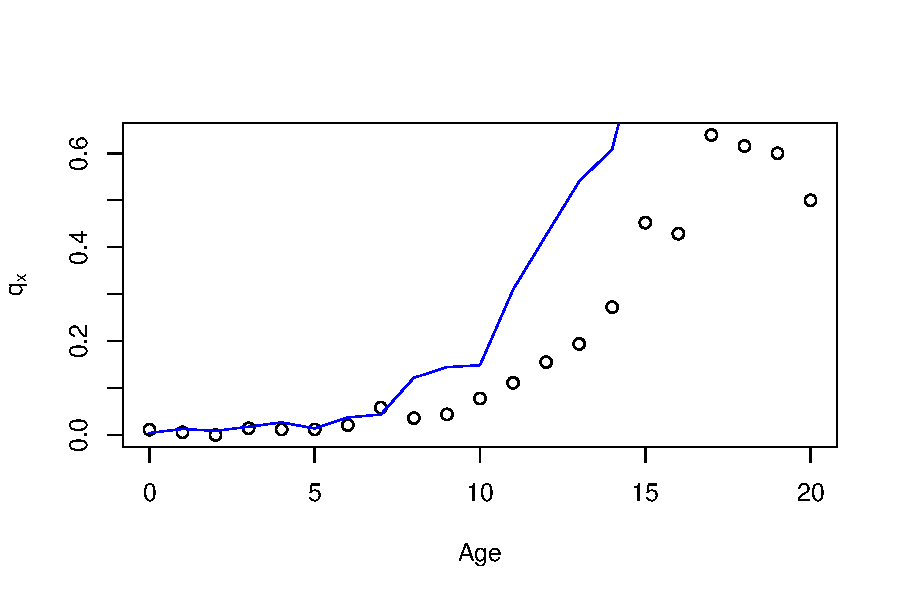
\includegraphics{LifeCon_files/figure-latex/unnamed-chunk-9-1} 

}

\caption{One-year Dog Mortality Rates, Blue Solid Line is for German Shepherds}\label{fig:unnamed-chunk-9}
\end{figure}

\textbf{Part B}

\begin{Shaded}
\begin{Highlighting}[]
\NormalTok{seqB1 <-}\StringTok{ }\KeywordTok{seq}\NormalTok{(}\DataTypeTok{from =} \DecValTok{0}\NormalTok{, }\DataTypeTok{to =} \DecValTok{20}\NormalTok{, }\DataTypeTok{by =} \FloatTok{0.25}\NormalTok{)}
\NormalTok{seqB2 <-}\StringTok{ }\NormalTok{seqB1 }\OperatorTok{+}\StringTok{ }\FloatTok{0.25}
\NormalTok{qxTerrB  <-}\StringTok{ }\NormalTok{(}\KeywordTok{summary}\NormalTok{(fitTerr,  }\DataTypeTok{time =}\NormalTok{ seqB1)}\OperatorTok{$}\NormalTok{surv }\OperatorTok{-}\StringTok{   }\KeywordTok{summary}\NormalTok{(fitTerr,  }\DataTypeTok{time =}\NormalTok{ seqB2)}\OperatorTok{$}\NormalTok{surv)   }\OperatorTok{/}\KeywordTok{summary}\NormalTok{(fitTerr,  }\DataTypeTok{time =}\NormalTok{ seqB1)}\OperatorTok{$}\NormalTok{surv}
\NormalTok{qxGShepB <-}\StringTok{ }\NormalTok{(}\KeywordTok{summary}\NormalTok{(fitGShep, }\DataTypeTok{time =}\NormalTok{ seqB1)}\OperatorTok{$}\NormalTok{surv }\OperatorTok{-}\StringTok{ }\KeywordTok{c}\NormalTok{(}\KeywordTok{summary}\NormalTok{(fitGShep, }\DataTypeTok{time =}\NormalTok{ seqB2)}\OperatorTok{$}\NormalTok{surv,}\DecValTok{0}\NormalTok{))}\OperatorTok{/}\KeywordTok{summary}\NormalTok{(fitGShep, }\DataTypeTok{time =}\NormalTok{ seqB1)}\OperatorTok{$}\NormalTok{surv}
\KeywordTok{plot}\NormalTok{(seqB1,qxTerrB, }\DataTypeTok{xlab =} \StringTok{"Age"}\NormalTok{, }\DataTypeTok{ylab =} \KeywordTok{expression}\NormalTok{(q[x]))}
\KeywordTok{lines}\NormalTok{(seqB1[}\DecValTok{1}\OperatorTok{:}\DecValTok{67}\NormalTok{], qxGShepB, }\DataTypeTok{col =} \StringTok{"blue"}\NormalTok{)}
\end{Highlighting}
\end{Shaded}

\begin{figure}

{\centering 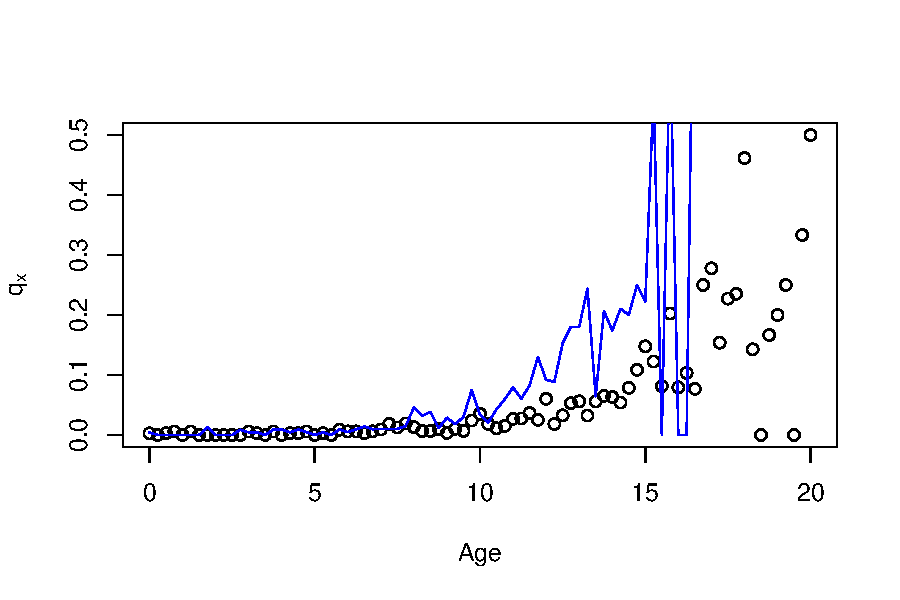
\includegraphics{LifeCon_files/figure-latex/unnamed-chunk-10-1} 

}

\caption{Quarterly Dog Mortality Rates, Blue Solid Line is for German Shepherds}\label{fig:unnamed-chunk-10}
\end{figure}

\textbf{Part C}

\begin{Shaded}
\begin{Highlighting}[]
\NormalTok{seqC1 <-}\StringTok{ }\KeywordTok{seq}\NormalTok{(}\DataTypeTok{from =} \DecValTok{0}\NormalTok{, }\DataTypeTok{to =} \DecValTok{20}\NormalTok{, }\DataTypeTok{by =} \DecValTok{2}\NormalTok{)}
\NormalTok{seqC2 <-}\StringTok{ }\NormalTok{seqC1 }\OperatorTok{+}\StringTok{ }\DecValTok{2}
\NormalTok{qxTerrC  <-}\StringTok{ }\NormalTok{(}\KeywordTok{summary}\NormalTok{(fitTerr,  }\DataTypeTok{time =}\NormalTok{ seqC1)}\OperatorTok{$}\NormalTok{surv }\OperatorTok{-}\StringTok{ }\KeywordTok{c}\NormalTok{(}\KeywordTok{summary}\NormalTok{(fitTerr,  }\DataTypeTok{time =}\NormalTok{ seqC2)}\OperatorTok{$}\NormalTok{surv,}\DecValTok{0}\NormalTok{))}\OperatorTok{/}\KeywordTok{summary}\NormalTok{(fitTerr,  }\DataTypeTok{time =}\NormalTok{ seqC1)}\OperatorTok{$}\NormalTok{surv}
\NormalTok{qxGShepC <-}\StringTok{ }\NormalTok{(}\KeywordTok{summary}\NormalTok{(fitGShep, }\DataTypeTok{time =}\NormalTok{ seqC1)}\OperatorTok{$}\NormalTok{surv }\OperatorTok{-}\StringTok{ }\KeywordTok{c}\NormalTok{(}\KeywordTok{summary}\NormalTok{(fitGShep, }\DataTypeTok{time =}\NormalTok{ seqC2)}\OperatorTok{$}\NormalTok{surv,}\DecValTok{0}\NormalTok{))}\OperatorTok{/}\KeywordTok{summary}\NormalTok{(fitGShep, }\DataTypeTok{time =}\NormalTok{ seqC1)}\OperatorTok{$}\NormalTok{surv}
\KeywordTok{plot}\NormalTok{(seqC1,qxTerrC, }\DataTypeTok{xlab =} \StringTok{"Age"}\NormalTok{, }\DataTypeTok{ylab =} \KeywordTok{expression}\NormalTok{(q[x]))}
\KeywordTok{lines}\NormalTok{(seqC1[}\DecValTok{1}\OperatorTok{:}\DecValTok{9}\NormalTok{], qxGShepC, }\DataTypeTok{col =} \StringTok{"blue"}\NormalTok{)}
\end{Highlighting}
\end{Shaded}

\begin{figure}

{\centering 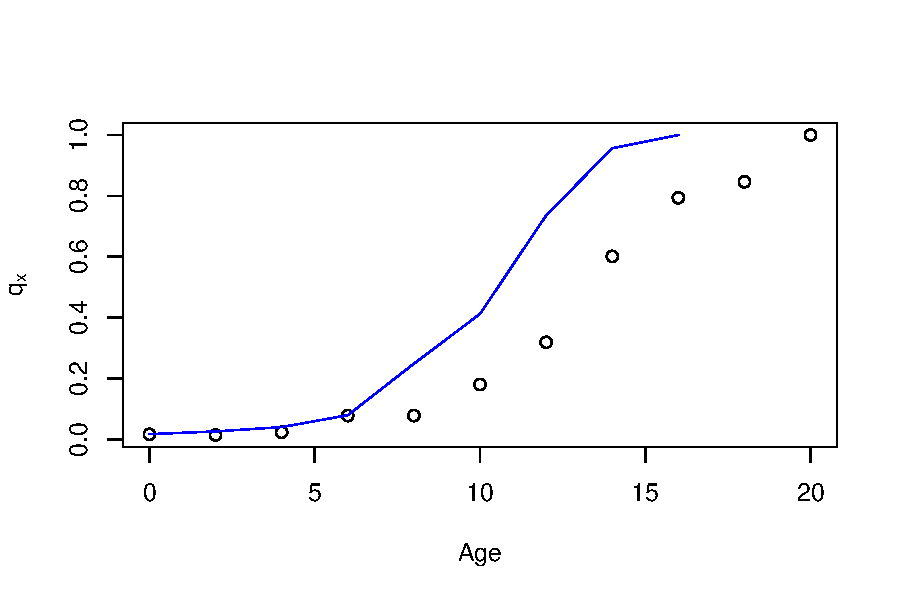
\includegraphics{LifeCon_files/figure-latex/unnamed-chunk-11-1} 

}

\caption{Two-year Dog Mortality Rates, Blue Solid Line is for German Shepherds}\label{fig:unnamed-chunk-11}
\end{figure}

\textbf{Part D}

\begin{Shaded}
\begin{Highlighting}[]
\NormalTok{DogAnn <-}\StringTok{ }\ControlFlowTok{function}\NormalTok{(}\DataTypeTok{x=}\NormalTok{x, }\DataTypeTok{q.x=}\NormalTok{qx)\{}
\NormalTok{  Term <-}\StringTok{ }\KeywordTok{length}\NormalTok{(q.x) }\OperatorTok{-}\StringTok{ }\NormalTok{(x}\OperatorTok{+}\DecValTok{1}\NormalTok{)}
\NormalTok{  kpx <-}\StringTok{ }\DecValTok{1} 
\NormalTok{  APV  <-}\StringTok{ }\DecValTok{0} 
 \ControlFlowTok{if}\NormalTok{ (Term}\OperatorTok{>}\DecValTok{0}\NormalTok{)\{ }\ControlFlowTok{for}\NormalTok{(k }\ControlFlowTok{in} \DecValTok{0}\OperatorTok{:}\NormalTok{(Term}\DecValTok{-1}\NormalTok{))\{ }
    \ControlFlowTok{if}\NormalTok{ (k}\OperatorTok{>}\DecValTok{1}\NormalTok{) \{kpx <-}\StringTok{ }\NormalTok{kpx}\OperatorTok{*}\NormalTok{(}\DecValTok{1}\OperatorTok{-}\NormalTok{q.x[x}\OperatorTok{+}\DecValTok{1}\OperatorTok{+}\NormalTok{k])\}}
\NormalTok{    APV  <-}\StringTok{ }\NormalTok{APV  }\OperatorTok{+}\StringTok{ }\NormalTok{kpx }\OperatorTok{*}\StringTok{  }\NormalTok{(}\DecValTok{1}\OperatorTok{/}\FloatTok{1.03}\NormalTok{)}\OperatorTok{^}\NormalTok{k   }\OperatorTok{*}\FloatTok{1.11}\OperatorTok{^}\NormalTok{k }\OperatorTok{*}\DecValTok{458}
\NormalTok{    \}\}}
 \KeywordTok{return}\NormalTok{(APV)}
\NormalTok{  \}}
\KeywordTok{DogAnn}\NormalTok{(}\DataTypeTok{x=}\DecValTok{2}\NormalTok{, }\DataTypeTok{q.x=}\NormalTok{qxTerrA)}
\KeywordTok{DogAnn}\NormalTok{(}\DataTypeTok{x=}\DecValTok{5}\NormalTok{, }\DataTypeTok{q.x=}\NormalTok{qxTerrA)}
\KeywordTok{DogAnn}\NormalTok{(}\DataTypeTok{x=}\DecValTok{12}\NormalTok{, }\DataTypeTok{q.x=}\NormalTok{qxTerrA)}
\KeywordTok{DogAnn}\NormalTok{(}\DataTypeTok{x=}\DecValTok{2}\NormalTok{, }\DataTypeTok{q.x=}\NormalTok{qxGShepA)}
\KeywordTok{DogAnn}\NormalTok{(}\DataTypeTok{x=}\DecValTok{5}\NormalTok{, }\DataTypeTok{q.x=}\NormalTok{qxGShepA)}
\KeywordTok{DogAnn}\NormalTok{(}\DataTypeTok{x=}\DecValTok{12}\NormalTok{, }\DataTypeTok{q.x=}\NormalTok{qxGShepA)}
\end{Highlighting}
\end{Shaded}

\begin{verbatim}
[1] 7605.312
[1] 5111.737
[1] 1795.301
[1] 5444.105
[1] 3420.25
[1] 1184.634
\end{verbatim}

Note that the mortality estimates in this exercise are based only on data for a specific breed. In contrast, the analysis in Section \ref{Sec:DogCostCare} used a Cox proportional hazards to regression model to use data from all breeds to form mortality estimates.

\begin{center}\rule{0.5\linewidth}{0.5pt}\end{center}

\hypertarget{appendix-data-dictionary}{%
\chapter{Appendix: Data Dictionary}\label{appendix-data-dictionary}}

This appendix describes the datasets used in this book.

For each set of data, we provide download buttons so that you can easily access the data in standard .csv (comma separated value) format. This allows you replicate and experiment with the methods developed in the book as well as sharpen your understanding through exercises.

We provide the source of each dataset. We also recommend, for deeper understanding, that you occasionally refer to these original sources to further develop your appreciation of the data underpinning the analytics developed in this book.

\hypertarget{Sec:DataUSPoPCounts}{%
\section{United States Population Mortality Counts}\label{Sec:DataUSPoPCounts}}

\textbf{Source}: The \href{https://www.mortality.org}{Human Mortality Database (HMD)}.

\textbf{Description}: We now bring into consideration \emph{mortality experience} for populations that had been observed over time, which is available at the \href{https://www.mortality.org}{Human Mortality Database (HMD)} for a wide range of countries. The available data include \emph{Exposures} by age, sex, and calender year period, i.e.~how many people of a given age and sex lived in the country's population during a given period of time, and corresponding \emph{Deaths}, i.e.~how many of these individuals had died.

The data are available using this download button:
Download the United States Population Mortality Counts Data

\begin{table}

\caption{\label{tab:unnamed-chunk-14}**US Population Mortality Counts First Five Rows**}
\centering
\begin{tabular}[t]{c|c|c|c|c|c}
\hline
Year\_start & Year\_end & Age & Female & Male & Total\\
\hline
1935 & 1939 & 0 & 4869267 & 5057569 & 9926836\\
\hline
1935 & 1939 & 1 & 4802597 & 4936238 & 9738835\\
\hline
1935 & 1939 & 2 & 5119574 & 5244634 & 10364208\\
\hline
1935 & 1939 & 3 & 5159494 & 5287402 & 10446896\\
\hline
1935 & 1939 & 4 & 5189350 & 5307754 & 10497104\\
\hline
\end{tabular}
\end{table}

\begin{table}

\caption{\label{tab:unnamed-chunk-14}**US Population Mortality Counts Last Five Rows**}
\centering
\begin{tabular}[t]{c|c|c|c|c|c}
\hline
Year\_start & Year\_end & Age & Female & Male & Total\\
\hline
2010 & 2014 & 106 & 3853.91 & 415.44 & 4269.35\\
\hline
2010 & 2014 & 107 & 2031.89 & 210.41 & 2242.30\\
\hline
2010 & 2014 & 108 & 1083.62 & 106.29 & 1189.91\\
\hline
2010 & 2014 & 109 & 535.32 & 58.42 & 593.73\\
\hline
2010 & 2014 & 110 & 576.06 & 80.03 & 656.09\\
\hline
\end{tabular}
\end{table}

\begin{table}

\caption{\label{tab:unnamed-chunk-15}**US Population Mortality Counts Summary Statistics**}
\centering
\begin{tabular}[t]{l|l|l|l|l|l|l}
\hline
  &   Year\_start &    Year\_end &      Age &     Female &      Male &     Total\\
\hline
 & Min.   :1935 & Min.   :1939 & Min.   :  0 & Min.   :      56 & Min.   :      21 & Min.   :      80\\
\hline
 & 1st Qu.:1954 & 1st Qu.:1958 & 1st Qu.: 27 & 1st Qu.: 1293833 & 1st Qu.:  823082 & 1st Qu.: 2130434\\
\hline
 & Median :1972 & Median :1976 & Median : 55 & Median : 5263300 & Median : 4850955 & Median :10124747\\
\hline
 & Mean   :1972 & Mean   :1976 & Mean   : 55 & Mean   : 4946072 & Mean   : 4758380 & Mean   : 9704453\\
\hline
 & 3rd Qu.:1991 & 3rd Qu.:1995 & 3rd Qu.: 83 & 3rd Qu.: 8238099 & 3rd Qu.: 8407376 & 3rd Qu.:16678945\\
\hline
 & Max.   :2010 & Max.   :2014 & Max.   :110 & Max.   :11606030 & Max.   :11674875 & Max.   :23280905\\
\hline
\end{tabular}
\end{table}

\hypertarget{Sec:SyntheticInsData}{%
\section{Synthetic Insurer Data}\label{Sec:SyntheticInsData}}

\textbf{Description}: We provide survival information for a hypothetical insurance company in \texttt{SyntheticInsurerData.csv}. The company has sold \emph{whole life insurance policies}, i.e.~policies that pay a \emph{death benefit} upon the policyholder's death, since 1955. Policyholders have to go through an underwriting examination, and in addition to policyholders' age, sex (0 for female, 1 for male), smoking status (0 for non-smoker, 1 for smoker), and the month of sale, the company records the applicants body-mass index (BMI) and the systolic blood pressure at the time of underwriting. Finally, for those policyholders with a claim, i.e., for the policyholders that have died, the company records the time of death (relative to the month of underwriting). The data are organized in the order of sales, so that the oldest entries are at the top of the data and the newest entries are at the bottom:

The data are available using this download button:
Download the Synthetic Insurer Data

\begin{table}

\caption{\label{tab:unnamed-chunk-16}**Synthetic Insurer First Five Rows**}
\centering
\begin{tabular}[t]{c|c|c|c|c|c|c|c}
\hline
Month\_of\_Sale & Age & Sex & Smoking & BMI & BloodPressure & Claim & Time\_of\_death\\
\hline
1 & 27 & 0 & 0 & 25.8 & 117 & YES & 55.63\\
\hline
1 & 51 & 1 & 0 & 17.6 & 109 & YES & 18.53\\
\hline
1 & 59 & 1 & 0 & 22.5 & 132 & YES & 15.88\\
\hline
1 & 37 & 1 & 0 & 22.9 & 109 & YES & 57.40\\
\hline
1 & 62 & 0 & 0 & 30.9 & 147 & YES & 27.83\\
\hline
\end{tabular}
\end{table}

\begin{table}

\caption{\label{tab:unnamed-chunk-16}**Synthetic Insurer Last Five Rows**}
\centering
\begin{tabular}[t]{c|c|c|c|c|c|c|c}
\hline
Month\_of\_Sale & Age & Sex & Smoking & BMI & BloodPressure & Claim & Time\_of\_death\\
\hline
780 & 57 & 1 & 1 & 19.30 & 118 & NO & NA\\
\hline
780 & 40 & 0 & 0 & 20.10 & 117 & NO & NA\\
\hline
780 & 27 & 1 & 0 & 20.60 & 90 & NO & NA\\
\hline
780 & 55 & 1 & 1 & 20.10 & 118 & NO & NA\\
\hline
780 & 23 & 1 & 0 & 19.03 & 82 & NO & NA\\
\hline
\end{tabular}
\end{table}

\begin{table}

\caption{\label{tab:unnamed-chunk-17}**Synthetic Insurer Summary Statistics**}
\centering
\begin{tabular}[t]{l|c|c|c|c}
\hline
  & Month\_of\_Sale &      Age &      Sex &    Smoking\\
\hline
 & Min.   :  1.0 & Min.   :19.00 & Min.   :0.0000 & Min.   :0.0000\\
\hline
 & 1st Qu.:209.0 & 1st Qu.:31.00 & 1st Qu.:0.0000 & 1st Qu.:0.0000\\
\hline
 & Median :382.0 & Median :39.00 & Median :1.0000 & Median :0.0000\\
\hline
 & Mean   :394.6 & Mean   :39.99 & Mean   :0.6988 & Mean   :0.2985\\
\hline
 & 3rd Qu.:591.0 & 3rd Qu.:48.00 & 3rd Qu.:1.0000 & 3rd Qu.:1.0000\\
\hline
 & Max.   :780.0 & Max.   :65.00 & Max.   :1.0000 & Max.   :1.0000\\
\hline
 &  &  &  & \\
\hline
\end{tabular}
\end{table}

\begin{table}
\centering
\begin{tabular}{l|c|c|c|c}
\hline
  &      BMI & BloodPressure & Claim & Time\_of\_death\\
\hline
 & Min.   :16.10 & Min.   : 57.0 & NO :101399 & Min.   : 0.00\\
\hline
 & 1st Qu.:19.50 & 1st Qu.:104.0 & YES: 59382 & 1st Qu.:17.99\\
\hline
 & Median :21.70 & Median :114.0 &  & Median :28.36\\
\hline
 & Mean   :22.79 & Mean   :114.7 &  & Mean   :28.27\\
\hline
 & 3rd Qu.:25.00 & 3rd Qu.:125.0 &  & 3rd Qu.:38.51\\
\hline
 & Max.   :69.60 & Max.   :208.0 &  & Max.   :64.20\\
\hline
 &  &  &  & NA's   :101399\\
\hline
\end{tabular}
\end{table}

\hypertarget{Sec:CanineMortality}{%
\section{Canine Mortality}\label{Sec:CanineMortality}}

\textbf{Source}: Canine mortality data are publicly available at \citet{pegram2021Data}. See \citet{pegram2021proportion} for additional background.

\textbf{Description}: In this dataset, there are 29865 observations used to study euthanasia. Our interest is in survival patterns by age and so we remove records where either the date of birth or death is missing or incorrect (we also removed 17 records with missing sex information); this results in 5933 records for analysis.

The data are available using this download button:
Download the Canine Mortality Data

\begin{table}

\caption{\label{tab:unnamed-chunk-18}**Canine Mortality First Five Rows**}
\centering
\begin{tabular}[t]{c|c|c|c|c|c|c|c}
\hline
animalid & Sex & Neutered & Breed & CauseDeath & Method.of.death & dateBirth & dateDeath\\
\hline
3534394 & Female & Entire & Boston Terrier & Disorder not diagnsosed & Euthanasia & 2016-02-02 & 2016-02-02\\
\hline
11836307 & Female & Entire & Bulldog & Behaviour disorder & Euthanasia & 2016-09-03 & 2016-09-03\\
\hline
12090746 & Male & Entire & Chinese Shar-Pei & Disorder not diagnsosed & Euthanasia & 2016-03-01 & 2016-03-01\\
\hline
12092145 & Female & Neutered & Crossbreed & Collapsed & Euthanasia & 2016-01-03 & 2016-01-03\\
\hline
11739930 & Female & Entire & German Shepherd Dog & Disorder not diagnsosed & Euthanasia & 2015-04-12 & 2015-04-12\\
\hline
\end{tabular}
\end{table}

\begin{table}

\caption{\label{tab:unnamed-chunk-18}**Canine Mortality Last Five Rows**}
\centering
\begin{tabular}[t]{c|c|c|c|c|c|c|c}
\hline
animalid & Sex & Neutered & Breed & CauseDeath & Method.of.death & dateBirth & dateDeath\\
\hline
11718193 & Female & Entire & Border Terrier & Heart disease & Euthanasia & 1998-12-03 & 2018-01-02\\
\hline
11514456 & Male & Entire & Jack Russell Terrier & Musculoskeletal disorder & Euthanasia & 1996-10-02 & 2016-10-02\\
\hline
6916114 & Female & Entire & Jack Russell Terrier & Disorder not diagnsosed & Euthanasia & 1996-06-09 & 2016-07-09\\
\hline
11542454 & Male & Neutered & Crossbreed & Disorder not diagnsosed & Unassisted & 1997-01-09 & 2017-02-12\\
\hline
3963609 & Male & Neutered & Jack Russell Terrier & Heart disease & Euthanasia & 1996-01-05 & 2017-01-09\\
\hline
\end{tabular}
\end{table}

\begin{table}

\caption{\label{tab:unnamed-chunk-19}**Canine Mortality Summary Statistics**}
\centering
\begin{tabular}[t]{l|c|c|c|c}
\hline
  &    animalid &     Sex &     Neutered &                        Breed\\
\hline
 & Min.   :  881900 & Female:2841 & Entire  :2529 & Crossbreed                :1259\\
\hline
 & 1st Qu.: 2401823 & Male  :3092 & Neutered:3404 & Staffordshire Bull Terrier: 507\\
\hline
 & Median : 6846177 &  &  & Labrador Retriever        : 481\\
\hline
 & Mean   : 6824982 &  &  & Jack Russell Terrier      : 352\\
\hline
 & 3rd Qu.:11559402 &  &  & German Shepherd Dog       : 234\\
\hline
 & Max.   :12493098 &  &  & Yorkshire Terrier         : 192\\
\hline
 &  &  &  & (Other)                   :2908\\
\hline
\end{tabular}
\end{table}

\begin{table}
\centering
\begin{tabular}{l|c|c|c|c}
\hline
  &                   CauseDeath &   Method.of.death &      dateBirth &      dateDeath\\
\hline
 & Disorder not diagnsosed:1126 & Euthanasia:5325 & 2005-01-03:  28 & 2016-12-12:  41\\
\hline
 & Collapsed              : 523 & Unassisted: 462 & 2005-01-05:  26 & 2016-10-07:  38\\
\hline
 & Neoplasia              : 522 & Unrecorded: 146 & 2004-01-01:  25 & 2016-08-09:  37\\
\hline
 & Mass                   : 375 &  & 2005-01-06:  25 & 2016-09-12:  37\\
\hline
 & Brain disorder         : 350 &  & 2003-01-05:  24 & 2016-11-09:  37\\
\hline
 & Behaviour disorder     : 341 &  & 2003-01-10:  24 & 2016-04-04:  35\\
\hline
 & (Other)                :2696 &  & (Other)   :5781 & (Other)   :5708\\
\hline
\end{tabular}
\end{table}

Show R Code to Pre-Process the Canine Mortality Data

\hypertarget{toggleCode.DataDict.1}{}
\begin{Shaded}
\begin{Highlighting}[]
\CommentTok{# Read in Revised Data}
\NormalTok{DogMortA <-}\StringTok{ }\KeywordTok{read.csv}\NormalTok{(}\StringTok{"Data/DogSurvivalData1.csv"}\NormalTok{)}
\NormalTok{DogMort <-}\StringTok{ }\NormalTok{DogMortA[,}\OperatorTok{-}\DecValTok{1}\NormalTok{]}
\NormalTok{DogMort}\OperatorTok{$}\NormalTok{dateBirth <-}\StringTok{ }\KeywordTok{as.Date}\NormalTok{(DogMort}\OperatorTok{$}\NormalTok{dateBirth, }\StringTok{"%Y-%m-%d"}\NormalTok{) }
\NormalTok{DogMort}\OperatorTok{$}\NormalTok{dateDeath <-}\StringTok{ }\KeywordTok{as.Date}\NormalTok{(DogMort}\OperatorTok{$}\NormalTok{dateDeath, }\StringTok{"%Y-%m-%d"}\NormalTok{)}
\NormalTok{DogMort}\OperatorTok{$}\NormalTok{AgeAtDeath <-}\StringTok{ }\NormalTok{(}\KeywordTok{as.numeric}\NormalTok{(DogMort}\OperatorTok{$}\NormalTok{dateDeath) }\OperatorTok{-}\StringTok{ }\KeywordTok{as.numeric}\NormalTok{(DogMort}\OperatorTok{$}\NormalTok{dateBirth))}\OperatorTok{/}\FloatTok{365.25}
\NormalTok{DogTerr <-}\StringTok{ }\KeywordTok{subset}\NormalTok{(DogMort, Breed }\OperatorTok{==}\StringTok{ "Jack Russell Terrier"}\NormalTok{)}
\NormalTok{DogGShep <-}\StringTok{ }\KeywordTok{subset}\NormalTok{(DogMort, Breed }\OperatorTok{==}\StringTok{ "German Shepherd Dog"}\NormalTok{)}
\end{Highlighting}
\end{Shaded}

\hypertarget{Sec:CanadianSelect}{%
\section{Canadian Female Select and Ultimate Mortality Table}\label{Sec:CanadianSelect}}

\textbf{Source}

\begin{itemize}
\tightlist
\item
  Individual Life Experience Subcommittee, ``Construction of CIA9704 Mortality Tables for Canadian Individual Insurance based on data from 1997 to 2004'', Canadian Institute of Actuaries (2010).
\item
  Accessed: October, 2021 from \url{http://www.cia-ica.ca/docs/default-source/2010/210028e.pdf}
\item
  Data retrieved from \url{https://mort.soa.org/} (Table 1458)
\end{itemize}

Select data are available using this download button:
Download the Canadian Female Select Mortality Table.

\begin{table}

\caption{\label{tab:unnamed-chunk-21}**Canadian Female Select Mortality First Five Rows**}
\centering
\begin{tabular}[t]{c|c|c|c|c|c|c|c}
\hline
Age & Select0 & Select1 & Select2 & Select3 & Select4 & Select5 & Select6\\
\hline
0 & 0.00035 & 0.00011 & 0.00011 & 1e-04 & 9e-05 & 9e-05 & 9e-05\\
\hline
1 & 0.00023 & 0.00011 & 0.00010 & 1e-04 & 9e-05 & 9e-05 & 9e-05\\
\hline
2 & 0.00011 & 0.00010 & 0.00010 & 9e-05 & 9e-05 & 9e-05 & 9e-05\\
\hline
3 & 0.00010 & 0.00010 & 0.00009 & 9e-05 & 9e-05 & 9e-05 & 9e-05\\
\hline
4 & 0.00010 & 0.00009 & 0.00009 & 9e-05 & 9e-05 & 9e-05 & 9e-05\\
\hline
\end{tabular}
\end{table}

\begin{tabular}{c|c|c|c|c|c|c|c}
\hline
Select7 & Select8 & Select9 & Select10 & Select11 & Select12 & Select13 & Select14\\
\hline
9e-05 & 0.00009 & 0.00009 & 0.00010 & 0.00010 & 0.00011 & 0.00012 & 0.00014\\
\hline
9e-05 & 0.00009 & 0.00009 & 0.00010 & 0.00011 & 0.00012 & 0.00013 & 0.00014\\
\hline
9e-05 & 0.00009 & 0.00010 & 0.00011 & 0.00012 & 0.00013 & 0.00014 & 0.00016\\
\hline
9e-05 & 0.00010 & 0.00011 & 0.00012 & 0.00013 & 0.00014 & 0.00016 & 0.00017\\
\hline
1e-04 & 0.00011 & 0.00012 & 0.00013 & 0.00014 & 0.00016 & 0.00017 & 0.00019\\
\hline
\end{tabular}

\begin{table}

\caption{\label{tab:unnamed-chunk-21}**Canadian Female Select Mortality Last Five Rows**}
\centering
\begin{tabular}[t]{c|c|c|c|c|c|c|c}
\hline
Age & Select0 & Select1 & Select2 & Select3 & Select4 & Select5 & Select6\\
\hline
76 & 0.00544 & 0.00819 & 0.01031 & 0.01236 & 0.01440 & 0.01799 & 0.02341\\
\hline
77 & 0.00566 & 0.00853 & 0.01073 & 0.01285 & 0.01633 & 0.02153 & 0.02751\\
\hline
78 & 0.00588 & 0.00887 & 0.01115 & 0.01457 & 0.01955 & 0.02530 & 0.03235\\
\hline
79 & 0.00609 & 0.00920 & 0.01264 & 0.01743 & 0.02298 & 0.02975 & 0.03791\\
\hline
80 & 0.00630 & 0.01043 & 0.01513 & 0.02049 & 0.02702 & 0.03486 & 0.04415\\
\hline
\end{tabular}
\end{table}

\begin{tabular}{c|c|c|c|c|c|c|c}
\hline
Select7 & Select8 & Select9 & Select10 & Select11 & Select12 & Select13 & Select14\\
\hline
0.02963 & 0.03723 & 0.04634 & 0.05706 & 0.06945 & 0.08367 & 0.09994 & 0.11842\\
\hline
0.03484 & 0.04363 & 0.05398 & 0.06599 & 0.07978 & 0.09560 & 0.11358 & 0.13176\\
\hline
0.04082 & 0.05082 & 0.06243 & 0.07580 & 0.09115 & 0.10864 & 0.12638 & 0.14378\\
\hline
0.04755 & 0.05877 & 0.07172 & 0.08661 & 0.10359 & 0.12088 & 0.13790 & 0.15707\\
\hline
0.05499 & 0.06751 & 0.08194 & 0.09843 & 0.11526 & 0.13190 & 0.15065 & 0.17193\\
\hline
\end{tabular}

Ultimate data are available using this download button:
Download the Canadian Female Ultimate Mortality Table.

\begin{table}

\caption{\label{tab:unnamed-chunk-22}**Canadian  Ultimate Mortality First Five Rows**}
\centering
\begin{tabular}[t]{c|c}
\hline
Age & qx\\
\hline
15 & 0.00015\\
\hline
16 & 0.00016\\
\hline
17 & 0.00018\\
\hline
18 & 0.00019\\
\hline
19 & 0.00021\\
\hline
\end{tabular}
\end{table}

\begin{table}

\caption{\label{tab:unnamed-chunk-22}**Canadian Ultimate Mortality Last Five Rows**}
\centering
\begin{tabular}[t]{c|c}
\hline
Age & qx\\
\hline
116 & 0.45\\
\hline
117 & 0.45\\
\hline
118 & 0.45\\
\hline
119 & 0.45\\
\hline
120 & 1.00\\
\hline
\end{tabular}
\end{table}

Show R Code to Pre-Process the Canadian Female Select and Ultimate Mortality Data

\hypertarget{toggleCode.DataDict.2}{}
\begin{Shaded}
\begin{Highlighting}[]
\NormalTok{CanadianSelect <-}\StringTok{ }\KeywordTok{read.csv}\NormalTok{(}\StringTok{"Data/CanadianFemaleSelectRead.csv"}\NormalTok{, }\DataTypeTok{stringsAsFactors =} \OtherTok{FALSE}\NormalTok{)}
\NormalTok{CanadianSelect1 <-}\StringTok{ }\KeywordTok{subset}\NormalTok{(CanadianSelect, Age }\OperatorTok{>=}\StringTok{ }\DecValTok{50} \OperatorTok{&}\StringTok{ }\NormalTok{Age }\OperatorTok{<=}\StringTok{ }\DecValTok{69}\NormalTok{)}
\NormalTok{CanadianSelect2 <-}\StringTok{ }\NormalTok{CanadianSelect1[}\DecValTok{2}\OperatorTok{:}\DecValTok{6}\NormalTok{,}\KeywordTok{c}\NormalTok{(}\DecValTok{1}\OperatorTok{:}\DecValTok{6}\NormalTok{,}\DecValTok{12}\NormalTok{,}\DecValTok{16}\NormalTok{)]}
\NormalTok{CanadianSelect3 <-}\StringTok{ }\NormalTok{CanadianSelect1[}\DecValTok{37}\OperatorTok{:}\DecValTok{41}\NormalTok{,}\DecValTok{1}\OperatorTok{:}\DecValTok{2}\NormalTok{]}
\NormalTok{CanadianSelect4 <-}\StringTok{ }\KeywordTok{cbind}\NormalTok{(CanadianSelect2,CanadianSelect3[,}\DecValTok{2}\NormalTok{],CanadianSelect3[,}\DecValTok{1}\NormalTok{])}
\KeywordTok{colnames}\NormalTok{(CanadianSelect4) <-}\StringTok{ }\KeywordTok{c}\NormalTok{(}\StringTok{"Age"}\NormalTok{, }\StringTok{"Select=0"}\NormalTok{,}\StringTok{"Select=1"}\NormalTok{,}\StringTok{"Select=2"}\NormalTok{,}\StringTok{"Select=3"}\NormalTok{,}\StringTok{"Select=4"}\NormalTok{,}\StringTok{"Select=10"}\NormalTok{,}\StringTok{"Select=14"}\NormalTok{, }\StringTok{"Ultimate Mortality"}\NormalTok{,}\StringTok{"Ultimate Age"}\NormalTok{ )}
\KeywordTok{rownames}\NormalTok{(CanadianSelect4) <-}\StringTok{ }\OtherTok{NULL}
\NormalTok{knitr}\OperatorTok{::}\KeywordTok{kable}\NormalTok{(CanadianSelect4, }\DataTypeTok{align =} \StringTok{"r"}\NormalTok{, }\DataTypeTok{caption=}\StringTok{"Select and Ultimate Female Canadian Mortality Rates"}\NormalTok{)}
\end{Highlighting}
\end{Shaded}

\hypertarget{Sec:KoreanMortality}{%
\section{Korean Mortality by Insured Status}\label{Sec:KoreanMortality}}

\textbf{Sources:}

\begin{itemize}
\tightlist
\item
  Insured lives and annuitant rates were drawn from a database organized by the Society of Actuaries, \url{https://mort.soa.org/}. These represent (beginning of the year) mortality rates (\(q_x\)).
\item
  The general population data are drawn from the \href{http://www.mortality.org/}{Human Mortality Database}. General population data are central death rates (\(m_x\)).
\end{itemize}

\hypertarget{korean-mortality---insured-lives}{%
\subsection*{Korean Mortality - Insured Lives}\label{korean-mortality---insured-lives}}
\addcontentsline{toc}{subsection}{Korean Mortality - Insured Lives}

The data are available using this download button:
Download the 2007 Korean Female Insured Lives Data.

\begin{table}

\caption{\label{tab:unnamed-chunk-25}**Korean Female Insured Lives First Five Rows**}
\centering
\begin{tabular}[t]{c|c}
\hline
Age & qx\\
\hline
0 & 0.00505\\
\hline
1 & 0.00044\\
\hline
2 & 0.00034\\
\hline
3 & 0.00025\\
\hline
4 & 0.00019\\
\hline
\end{tabular}
\end{table}

\begin{table}

\caption{\label{tab:unnamed-chunk-25}**Korean Female Insured Lives Last Five Rows**}
\centering
\begin{tabular}[t]{c|c}
\hline
Age & qx\\
\hline
108 & 0.76028\\
\hline
109 & 0.80509\\
\hline
110 & 0.84620\\
\hline
111 & 0.88274\\
\hline
112 & 1.00000\\
\hline
\end{tabular}
\end{table}

\hypertarget{korean-mortality---annuitants}{%
\subsection*{Korean Mortality - Annuitants}\label{korean-mortality---annuitants}}
\addcontentsline{toc}{subsection}{Korean Mortality - Annuitants}

The data are available using this download button:
Download the 2007 Korean Female Annuitants Data.

\begin{table}

\caption{\label{tab:unnamed-chunk-27}**Korean Female Annuitant First Five Rows**}
\centering
\begin{tabular}[t]{c|c}
\hline
Age & qx\\
\hline
45 & 0.00037\\
\hline
46 & 0.00041\\
\hline
47 & 0.00045\\
\hline
48 & 0.00048\\
\hline
49 & 0.00051\\
\hline
\end{tabular}
\end{table}

\begin{table}

\caption{\label{tab:unnamed-chunk-27}**Korean Female Annuitant Last Five Rows**}
\centering
\begin{tabular}[t]{c|c}
\hline
Age & qx\\
\hline
108 & 0.66236\\
\hline
109 & 0.71596\\
\hline
110 & 0.76430\\
\hline
111 & 0.80563\\
\hline
112 & 1.00000\\
\hline
\end{tabular}
\end{table}

\hypertarget{korean-mortality---population}{%
\subsection*{Korean Mortality - Population}\label{korean-mortality---population}}
\addcontentsline{toc}{subsection}{Korean Mortality - Population}

The data are available using this download button:
Download the Korean Population Mortality Data.

\begin{table}

\caption{\label{tab:unnamed-chunk-29}**Korean Female Population First Five Rows**}
\centering
\begin{tabular}[t]{c|c|c|c|c}
\hline
Year & Age & Female & Male & Total\\
\hline
2003 & 0 & 0.004846 & 0.005998 & 0.005447\\
\hline
2003 & 1 & 0.000477 & 0.000418 & 0.000446\\
\hline
2003 & 2 & 0.000291 & 0.000409 & 0.000353\\
\hline
2003 & 3 & 0.000286 & 0.00031 & 0.000298\\
\hline
2003 & 4 & 0.000261 & 0.000347 & 0.000306\\
\hline
\end{tabular}
\end{table}

\begin{table}

\caption{\label{tab:unnamed-chunk-29}**Korean Female Population Last Five Rows**}
\centering
\begin{tabular}[t]{c|c|c|c|c}
\hline
Year & Age & Female & Male & Total\\
\hline
2018 & 106 & 0.556191 & 0.667144 & 0.570571\\
\hline
2018 & 107 & 0.615315 & 0.848961 & 0.642871\\
\hline
2018 & 108 & 0.698276 & 1.426573 & 0.761357\\
\hline
2018 & 109 & 0.874699 & 4.285714 & 1.003864\\
\hline
2018 & 110 & 1.804822 & . & 1.804822\\
\hline
\end{tabular}
\end{table}

\hypertarget{Sec:MortalityCountry}{%
\section{Mortality by Country}\label{Sec:MortalityCountry}}

\textbf{Source:} The \href{http://www.mortality.org/}{Human Mortality Database}. In addition to classification by country, we also look at experience by sex and age as these distinctions are well known. General population data are central death rates (\(m_x\)).

\hypertarget{population-mortality---japan}{%
\subsection*{Population Mortality - Japan}\label{population-mortality---japan}}
\addcontentsline{toc}{subsection}{Population Mortality - Japan}

The data are available using this download button:
Download the Japan Population Mortality Data.

\begin{table}

\caption{\label{tab:unnamed-chunk-31}**Japan Population  First Five Rows**}
\centering
\begin{tabular}[t]{c|c|c|c|c}
\hline
Year & Age & Female & Male & Total\\
\hline
1947 & 0 & 0.083595 & 0.095448 & 0.089645\\
\hline
1947 & 1 & 0.035643 & 0.037017 & 0.036341\\
\hline
1947 & 2 & 0.017271 & 0.017203 & 0.017237\\
\hline
1947 & 3 & 0.011227 & 0.01133 & 0.011279\\
\hline
1947 & 4 & 0.007023 & 0.007468 & 0.007248\\
\hline
\end{tabular}
\end{table}

\begin{table}

\caption{\label{tab:unnamed-chunk-31}**Japan Population  Last Five Rows**}
\centering
\begin{tabular}[t]{c|c|c|c|c}
\hline
Year & Age & Female & Male & Total\\
\hline
2019 & 106 & 0.522855 & 0.69263 & 0.537623\\
\hline
2019 & 107 & 0.534649 & 0.66628 & 0.544456\\
\hline
2019 & 108 & 0.569069 & 0.607969 & 0.571733\\
\hline
2019 & 109 & 0.608248 & 0.806337 & 0.619736\\
\hline
2019 & 110 & 0.630664 & 0.927907 & 0.643787\\
\hline
\end{tabular}
\end{table}

\hypertarget{population-mortality---poland}{%
\subsection*{Population Mortality - Poland}\label{population-mortality---poland}}
\addcontentsline{toc}{subsection}{Population Mortality - Poland}

The data are available using this download button:
Download the Poland Population Mortality Data.

\begin{table}

\caption{\label{tab:unnamed-chunk-33}**Poland  Population  First Five Rows**}
\centering
\begin{tabular}[t]{c|c|c|c|c}
\hline
Year & Age & Female & Male & Total\\
\hline
1958 & 0 & 0.065617 & 0.08371 & 0.074886\\
\hline
1958 & 1 & 0.004736 & 0.005034 & 0.004888\\
\hline
1958 & 2 & 0.001734 & 0.002034 & 0.001888\\
\hline
1958 & 3 & 0.001191 & 0.001463 & 0.00133\\
\hline
1958 & 4 & 0.000853 & 0.001073 & 0.000965\\
\hline
\end{tabular}
\end{table}

\begin{table}

\caption{\label{tab:unnamed-chunk-33}**Poland  Population  Last Five Rows**}
\centering
\begin{tabular}[t]{c|c|c|c|c}
\hline
Year & Age & Female & Male & Total\\
\hline
2019 & 106 & 0.423814 & 0.307903 & 0.404767\\
\hline
2019 & 107 & 0.394572 & 0.350672 & 0.387116\\
\hline
2019 & 108 & 0.657174 & 0.760938 & 0.673882\\
\hline
2019 & 109 & 0.529723 & 0 & 0.449214\\
\hline
2019 & 110 & 1.753104 & 0 & 1.517067\\
\hline
\end{tabular}
\end{table}

\hypertarget{population-mortality---united-states}{%
\subsection*{Population Mortality - United States}\label{population-mortality---united-states}}
\addcontentsline{toc}{subsection}{Population Mortality - United States}

The data are available using this download button:
Download the USA Population Mortality Data.

\begin{table}

\caption{\label{tab:unnamed-chunk-35}**USA Population  First Five Rows**}
\centering
\begin{tabular}[t]{c|c|c|c|c}
\hline
Year & Age & Female & Male & Total\\
\hline
1933 & 0 & 0.054177 & 0.068175 & 0.061292\\
\hline
1933 & 1 & 0.008866 & 0.010039 & 0.009459\\
\hline
1933 & 2 & 0.004025 & 0.004671 & 0.004351\\
\hline
1933 & 3 & 0.002869 & 0.003333 & 0.003104\\
\hline
1933 & 4 & 0.002230 & 0.002537 & 0.002386\\
\hline
\end{tabular}
\end{table}

\begin{table}

\caption{\label{tab:unnamed-chunk-35}**USA Population Last Five Rows**}
\centering
\begin{tabular}[t]{c|c|c|c|c}
\hline
Year & Age & Female & Male & Total\\
\hline
2019 & 106 & 0.517094 & 0.521663 & 0.517643\\
\hline
2019 & 107 & 0.509637 & 0.586390 & 0.518399\\
\hline
2019 & 108 & 0.637707 & 0.724113 & 0.647031\\
\hline
2019 & 109 & 0.550384 & 0.373599 & 0.531748\\
\hline
2019 & 110 & 0.598467 & 0.509626 & 0.588324\\
\hline
\end{tabular}
\end{table}

Show R Code to Pre-Process the Mortality Data by Country

\hypertarget{toggleCode.DataCountry.2}{}
\begin{Shaded}
\begin{Highlighting}[]
\NormalTok{JapanPopFemaleqx  <-}\StringTok{ }\KeywordTok{as.numeric}\NormalTok{(JapanPop2019}\OperatorTok{$}\NormalTok{Female) }\OperatorTok{/}\NormalTok{(}\DecValTok{1} \OperatorTok{+}\StringTok{ }\KeywordTok{as.numeric}\NormalTok{(JapanPop2019}\OperatorTok{$}\NormalTok{Female) }\OperatorTok{/}\DecValTok{2}\NormalTok{)}
\NormalTok{JapanPopMaleqx    <-}\StringTok{ }\KeywordTok{as.numeric}\NormalTok{(JapanPop2019}\OperatorTok{$}\NormalTok{Male)   }\OperatorTok{/}\NormalTok{(}\DecValTok{1} \OperatorTok{+}\StringTok{ }\KeywordTok{as.numeric}\NormalTok{(JapanPop2019}\OperatorTok{$}\NormalTok{Male)   }\OperatorTok{/}\DecValTok{2}\NormalTok{)}
\NormalTok{PolandPopFemaleqx <-}\StringTok{ }\KeywordTok{as.numeric}\NormalTok{(PolandPop2019}\OperatorTok{$}\NormalTok{Female)}\OperatorTok{/}\NormalTok{(}\DecValTok{1} \OperatorTok{+}\StringTok{ }\KeywordTok{as.numeric}\NormalTok{(PolandPop2019}\OperatorTok{$}\NormalTok{Female)}\OperatorTok{/}\DecValTok{2}\NormalTok{)}
\NormalTok{PolandPopMaleqx   <-}\StringTok{ }\KeywordTok{as.numeric}\NormalTok{(PolandPop2019}\OperatorTok{$}\NormalTok{Male)  }\OperatorTok{/}\NormalTok{(}\DecValTok{1} \OperatorTok{+}\StringTok{ }\KeywordTok{as.numeric}\NormalTok{(PolandPop2019}\OperatorTok{$}\NormalTok{Male)  }\OperatorTok{/}\DecValTok{2}\NormalTok{)}
\NormalTok{USAPopFemaleqx    <-}\StringTok{ }\KeywordTok{as.numeric}\NormalTok{(USAPop2019}\OperatorTok{$}\NormalTok{Female)   }\OperatorTok{/}\NormalTok{(}\DecValTok{1} \OperatorTok{+}\StringTok{ }\KeywordTok{as.numeric}\NormalTok{(USAPop2019}\OperatorTok{$}\NormalTok{Female)   }\OperatorTok{/}\DecValTok{2}\NormalTok{)}
\NormalTok{USAPopMaleqx      <-}\StringTok{ }\KeywordTok{as.numeric}\NormalTok{(USAPop2019}\OperatorTok{$}\NormalTok{Male)     }\OperatorTok{/}\NormalTok{(}\DecValTok{1} \OperatorTok{+}\StringTok{ }\KeywordTok{as.numeric}\NormalTok{(USAPop2019}\OperatorTok{$}\NormalTok{Male)     }\OperatorTok{/}\DecValTok{2}\NormalTok{)}

\NormalTok{PolandPopMaleqx[}\DecValTok{110}\NormalTok{] <-}\StringTok{ }\DecValTok{1}\NormalTok{ ->}\StringTok{ }\NormalTok{PolandPopMaleqx[}\DecValTok{111}\NormalTok{]}

\NormalTok{IntlMort <-}\StringTok{ }\KeywordTok{data.frame}\NormalTok{(}\KeywordTok{cbind}\NormalTok{(JapanPop2019}\OperatorTok{$}\NormalTok{Age, JapanPopFemaleqx, JapanPopMaleqx, PolandPopFemaleqx,}
\NormalTok{                             PolandPopMaleqx, USAPopFemaleqx, USAPopMaleqx))}
\KeywordTok{names}\NormalTok{(IntlMort) <-}\StringTok{ }\KeywordTok{c}\NormalTok{(}\StringTok{"Age"}\NormalTok{, }\StringTok{"qx_Female_Japan"}\NormalTok{, }\StringTok{"qx_Male_Japan"}\NormalTok{, }\StringTok{"qx_Female_Poland"}\NormalTok{, }
                            \StringTok{"qx_Male_Poland"}\NormalTok{,  }\StringTok{"qx_Female_USA"}\NormalTok{, }\StringTok{"qx_Male_USA"}\NormalTok{)}
\CommentTok{#str(IntlMort)}
\end{Highlighting}
\end{Shaded}

\hypertarget{Sec:DataDisIncome}{%
\section{Disability Income}\label{Sec:DataDisIncome}}

\textbf{Source:} \citet{zayatz2015social}, Tables 14A, 14B, 21A, 21B

\textbf{Description}:

\begin{itemize}
\tightlist
\item
  Entitlement age \texttt{Entryx} denotes age last birthday at entitlement to disability benefits.
\item
  The duration \texttt{Select.y} is measured in years since entitlement.
\item
  Attained age \texttt{Attainedx} is calculated as sum of \texttt{Entryx} and duration.
\item
  The select and ultimate table is read across the row for 0-10 years of entitlement, and down the last (ultimate) column for 10 or more years of entitlement.
\end{itemize}

\hypertarget{disability-recovery-rates---male}{%
\subsection*{Disability Recovery Rates - Male}\label{disability-recovery-rates---male}}
\addcontentsline{toc}{subsection}{Disability Recovery Rates - Male}

The data are available using this download button:
Download the Male Disability Recovery Rates Data

\begin{table}

\caption{\label{tab:unnamed-chunk-38}**Male Disability Recovery Rates First Five Rows**}
\centering
\begin{tabular}[t]{c|c|c|c|c|c|c}
\hline
Entryx & Select.0 & Select.1 & Select.2 & Select.3 & Select.4 & Select.5\\
\hline
16 & 0.009456 & 0.021605 & 0.022333 & 0.012668 & 0.076435 & 0.102141\\
\hline
17 & 0.008263 & 0.016584 & 0.014498 & 0.012572 & 0.069437 & 0.087636\\
\hline
18 & 0.006705 & 0.012183 & 0.008357 & 0.013495 & 0.058735 & 0.069197\\
\hline
19 & 0.004731 & 0.008923 & 0.006305 & 0.013196 & 0.046345 & 0.052405\\
\hline
20 & 0.003801 & 0.007313 & 0.005540 & 0.012486 & 0.037918 & 0.043175\\
\hline
\end{tabular}
\end{table}

\begin{tabular}{c|c|c|c|c|c}
\hline
Select.6 & Select.7 & Select.8 & Select.9 & Ultimate & Attainedx\\
\hline
0.112060 & 0.075165 & 0.056866 & 0.056944 & 0.040505 & 26\\
\hline
0.087495 & 0.063740 & 0.050628 & 0.048795 & 0.035679 & 27\\
\hline
0.062385 & 0.051173 & 0.043173 & 0.038157 & 0.030488 & 28\\
\hline
0.047538 & 0.040872 & 0.035954 & 0.030026 & 0.025868 & 29\\
\hline
0.038960 & 0.032915 & 0.029194 & 0.022511 & 0.020527 & 30\\
\hline
\end{tabular}

\begin{table}

\caption{\label{tab:unnamed-chunk-38}**Male Disability Recovery Rates Last Five Rows**}
\centering
\begin{tabular}[t]{c|c|c|c|c|c|c}
\hline
Entryx & Select.0 & Select.1 & Select.2 & Select.3 & Select.4 & Select.5\\
\hline
60 & 0.000623 & 0.000626 & 0.000110 & 0.000793 & 0.001620 & 0.001171\\
\hline
61 & 0.000475 & 0.000229 & 0.000088 & 0.000624 & 0.001386 & NA\\
\hline
62 & 0.000260 & 0.000164 & 0.000070 & 0.000265 & NA & NA\\
\hline
63 & 0.000250 & 0.000241 & 0.000109 & NA & NA & NA\\
\hline
64 & 0.000259 & 0.000297 & NA & NA & NA & NA\\
\hline
\end{tabular}
\end{table}

\begin{tabular}{c|c|c|c|c|c}
\hline
Select.6 & Select.7 & Select.8 & Select.9 & Ultimate & Attainedx\\
\hline
NA & NA & NA & NA & NA & 70\\
\hline
NA & NA & NA & NA & NA & 71\\
\hline
NA & NA & NA & NA & NA & 72\\
\hline
NA & NA & NA & NA & NA & 73\\
\hline
NA & NA & NA & NA & NA & NA\\
\hline
\end{tabular}

\hypertarget{disability-recovery-rates---female}{%
\subsection*{Disability Recovery Rates - FeMale}\label{disability-recovery-rates---female}}
\addcontentsline{toc}{subsection}{Disability Recovery Rates - FeMale}

The data are available using this download button:
Download the Female Disability Recovery Rates Data

\begin{table}

\caption{\label{tab:unnamed-chunk-39}**Female Disability Recovery Rates First Five Rows**}
\centering
\begin{tabular}[t]{c|c|c|c|c|c|c}
\hline
Entryx & Select.0 & Select.1 & Select.2 & Select.3 & Select.4 & Select.5\\
\hline
16 & 0.012151 & 0.018994 & 0.014082 & 0.012065 & 0.047060 & 0.072175\\
\hline
17 & 0.009336 & 0.014397 & 0.009586 & 0.010991 & 0.046968 & 0.061956\\
\hline
18 & 0.006091 & 0.010576 & 0.007151 & 0.011074 & 0.044637 & 0.049647\\
\hline
19 & 0.003622 & 0.008175 & 0.005680 & 0.010073 & 0.036436 & 0.038087\\
\hline
20 & 0.003286 & 0.006613 & 0.005661 & 0.009786 & 0.029334 & 0.035754\\
\hline
\end{tabular}
\end{table}

\begin{tabular}{c|c|c|c|c|c}
\hline
Select.6 & Select.7 & Select.8 & Select.9 & Ultimate & Attainedx\\
\hline
0.076092 & 0.068259 & 0.070327 & 0.060100 & 0.047138 & 26\\
\hline
0.064836 & 0.058914 & 0.060321 & 0.049663 & 0.038233 & 27\\
\hline
0.053373 & 0.049032 & 0.048837 & 0.037076 & 0.030978 & 28\\
\hline
0.040477 & 0.039143 & 0.039245 & 0.028696 & 0.025747 & 29\\
\hline
0.034821 & 0.030852 & 0.030893 & 0.023135 & 0.020749 & 30\\
\hline
\end{tabular}

\begin{table}

\caption{\label{tab:unnamed-chunk-39}**Female Disability Recovery Rates Last Five Rows**}
\centering
\begin{tabular}[t]{c|c|c|c|c|c|c}
\hline
Entryx & Select.0 & Select.1 & Select.2 & Select.3 & Select.4 & Select.5\\
\hline
61 & 0.000425 & 0.000412 & 0.000138 & 0.000715 & 0.001145 & NA\\
\hline
62 & 0.000141 & 0.000276 & 0.000143 & 0.000267 & NA & NA\\
\hline
63 & 0.000203 & 0.000255 & 0.000084 & NA & NA & NA\\
\hline
64 & 0.000222 & 0.000223 & NA & NA & NA & NA\\
\hline
65 & 0.000212 & NA & NA & NA & NA & NA\\
\hline
\end{tabular}
\end{table}

\begin{tabular}{c|c|c|c|c|c}
\hline
Select.6 & Select.7 & Select.8 & Select.9 & Ultimate & Attainedx\\
\hline
NA & NA & NA & NA & NA & 71\\
\hline
NA & NA & NA & NA & NA & 72\\
\hline
NA & NA & NA & NA & NA & 73\\
\hline
NA & NA & NA & NA & NA & 74\\
\hline
NA & NA & NA & NA & NA & 75\\
\hline
\end{tabular}

\hypertarget{death-and-disability-recovery-rates---male}{%
\subsection*{Death and Disability Recovery Rates - Male}\label{death-and-disability-recovery-rates---male}}
\addcontentsline{toc}{subsection}{Death and Disability Recovery Rates - Male}

The data are available using this download button:
Download the Male Death and Disability Recovery Rates Data

\begin{table}

\caption{\label{tab:unnamed-chunk-40}**Male Death and Disability Recovery Rates First Five Rows**}
\centering
\begin{tabular}[t]{c|c|c|c|c|c|c}
\hline
Entryx & Select.0 & Select.1 & Select.2 & Select.3 & Select.4 & Select.5\\
\hline
16 & 0.013461 & 0.028723 & 0.027576 & 0.018476 & 0.080463 & 0.104575\\
\hline
17 & 0.013996 & 0.024853 & 0.020698 & 0.019304 & 0.074251 & 0.092377\\
\hline
18 & 0.014013 & 0.021066 & 0.015289 & 0.020650 & 0.064944 & 0.076273\\
\hline
19 & 0.014643 & 0.017300 & 0.013588 & 0.020882 & 0.052550 & 0.058905\\
\hline
20 & 0.013950 & 0.015959 & 0.012445 & 0.020439 & 0.044388 & 0.049337\\
\hline
\end{tabular}
\end{table}

\begin{tabular}{c|c|c|c|c|c}
\hline
Select.6 & Select.7 & Select.8 & Select.9 & Ultimate & Attainedx\\
\hline
0.121258 & 0.082287 & 0.062582 & 0.063157 & 0.048641 & 26\\
\hline
0.094508 & 0.070856 & 0.057023 & 0.054308 & 0.042584 & 27\\
\hline
0.067078 & 0.057816 & 0.049906 & 0.043654 & 0.036840 & 28\\
\hline
0.052107 & 0.046330 & 0.043202 & 0.035403 & 0.031748 & 29\\
\hline
0.043401 & 0.039036 & 0.036866 & 0.027852 & 0.026635 & 30\\
\hline
\end{tabular}

\begin{table}

\caption{\label{tab:unnamed-chunk-40}**Male Death and Disability Recovery Rates Last Five Rows**}
\centering
\begin{tabular}[t]{c|c|c|c|c|c|c}
\hline
Entryx & Select.0 & Select.1 & Select.2 & Select.3 & Select.4 & Select.5\\
\hline
61 & 0.074628 & 0.049784 & 0.041770 & 0.040088 & 0.040294 & 0.043873\\
\hline
62 & 0.081799 & 0.054262 & 0.044259 & 0.043029 & 0.045562 & 0.045980\\
\hline
63 & 0.095675 & 0.064214 & 0.051854 & 0.050283 & 0.050324 & 0.054444\\
\hline
64 & 0.115280 & 0.070667 & 0.055579 & 0.055825 & 0.056144 & 0.062203\\
\hline
65 & 0.124020 & 0.074767 & 0.055770 & 0.060810 & 0.060725 & 0.062011\\
\hline
\end{tabular}
\end{table}

\begin{tabular}{c|c|c|c|c|c}
\hline
Select.6 & Select.7 & Select.8 & Select.9 & Ultimate & Attainedx\\
\hline
0.047364 & 0.048433 & 0.052576 & 0.054822 & 0.061678 & 71\\
\hline
0.049717 & 0.052812 & 0.055874 & 0.057919 & 0.065458 & 72\\
\hline
0.056046 & 0.060056 & 0.065220 & 0.065203 & 0.069131 & 73\\
\hline
0.061766 & 0.064501 & 0.073359 & 0.073558 & 0.073835 & 74\\
\hline
0.064728 & 0.066258 & 0.081121 & 0.081981 & 0.079210 & 75\\
\hline
\end{tabular}

\hypertarget{death-and-disability-recovery-rates---female}{%
\subsection*{Death and Disability Recovery Rates - Female}\label{death-and-disability-recovery-rates---female}}
\addcontentsline{toc}{subsection}{Death and Disability Recovery Rates - Female}

The data are available using this download button:
Download the Female Death and Disability Recovery Rates Data

\begin{table}

\caption{\label{tab:unnamed-chunk-41}**Female Death and Disability Recovery Rates First Five Rows**}
\centering
\begin{tabular}[t]{c|c|c|c|c|c|c}
\hline
Entryx & Select.0 & Select.1 & Select.2 & Select.3 & Select.4 & Select.5\\
\hline
16 & 0.014809 & 0.023141 & 0.017968 & 0.017366 & 0.049789 & 0.075158\\
\hline
17 & 0.014491 & 0.020749 & 0.014300 & 0.016203 & 0.050781 & 0.066032\\
\hline
18 & 0.013639 & 0.018872 & 0.012580 & 0.016785 & 0.049449 & 0.054591\\
\hline
19 & 0.013372 & 0.016900 & 0.011715 & 0.015952 & 0.042374 & 0.042293\\
\hline
20 & 0.012495 & 0.015506 & 0.011147 & 0.016198 & 0.034865 & 0.040256\\
\hline
\end{tabular}
\end{table}

\begin{tabular}{c|c|c|c|c|c}
\hline
Select.6 & Select.7 & Select.8 & Select.9 & Ultimate & Attainedx\\
\hline
0.080785 & 0.077056 & 0.076726 & 0.063991 & 0.053156 & 26\\
\hline
0.070660 & 0.066819 & 0.065950 & 0.054640 & 0.044335 & 27\\
\hline
0.060112 & 0.056380 & 0.053425 & 0.043089 & 0.036942 & 28\\
\hline
0.047345 & 0.046225 & 0.044149 & 0.035500 & 0.032151 & 29\\
\hline
0.041520 & 0.036651 & 0.036679 & 0.030169 & 0.028106 & 30\\
\hline
\end{tabular}

\begin{table}

\caption{\label{tab:unnamed-chunk-41}**Female Death and Disability Recovery Rates Last Five Rows**}
\centering
\begin{tabular}[t]{c|c|c|c|c|c|c}
\hline
Entryx & Select.0 & Select.1 & Select.2 & Select.3 & Select.4 & Select.5\\
\hline
61 & 0.062420 & 0.042505 & 0.033209 & 0.031489 & 0.028894 & 0.032939\\
\hline
62 & 0.067121 & 0.048084 & 0.038302 & 0.033147 & 0.034093 & 0.034971\\
\hline
63 & 0.079963 & 0.055521 & 0.041415 & 0.040768 & 0.037425 & 0.040520\\
\hline
64 & 0.100669 & 0.060609 & 0.049733 & 0.043582 & 0.046125 & 0.044295\\
\hline
65 & 0.108699 & 0.068326 & 0.056379 & 0.046410 & 0.051687 & 0.045036\\
\hline
\end{tabular}
\end{table}

\begin{tabular}{c|c|c|c|c|c}
\hline
Select.6 & Select.7 & Select.8 & Select.9 & Ultimate & Attainedx\\
\hline
0.032992 & 0.036253 & 0.039311 & 0.041570 & 0.043767 & 71\\
\hline
0.036726 & 0.038876 & 0.042402 & 0.045475 & 0.046781 & 72\\
\hline
0.043163 & 0.043178 & 0.048631 & 0.048940 & 0.050292 & 73\\
\hline
0.049059 & 0.049045 & 0.054979 & 0.055358 & 0.053434 & 74\\
\hline
0.053099 & 0.054934 & 0.061211 & 0.061746 & 0.057982 & 75\\
\hline
\end{tabular}

\hypertarget{test-a-few-things}{%
\subsubsection*{Test a few things}\label{test-a-few-things}}
\addcontentsline{toc}{subsubsection}{Test a few things}

Access from Github instead of OneDrive???

Access button
Access the Canadian Female Select and Ultimate Mortality Table Github .

Then, do a ``File==\textgreater{} Save As'' to download the data\ldots.

Time taken for this draft of the book: 0.12 minutes.

  \bibliography{References/LDAReference2020A.bib,References/ContPayment.bib}

\end{document}
